%
% Draft  paper
%  Merino Evolution, Skin Characteristics and Fleece Quality
%
 
\documentclass[titlepage]{article}  % Latex2e
\usepackage{graphicx,lscape,subfigure}
 

\title{ Merino Evolution, Skin Characteristics and Fleece Quality}
\author{Neville Jackson,\thanks{The scientific theories and interpretations 
of data in this report are those of the authors only and are not necessarily 
associated with CSIRO or its stakeholders.}
I. G. Maddocks, 
J. Lax,
G.P.M.Moore,
and J.E.Watts.}
\date{Sep 4, 1990}   % Deleting this command produces today's date.


 
\begin{document} 
 
\maketitle      
\tableofcontents

\clearpage
\section{Acknowledgement}
    We would like to thank the studmasters who have cooperated in providing
access to sheep and facilities for this study.  Part of the work was supported
by a research grant from the Bicentennial Research Fund of the NSW Branch of
the Australian Association of Stud Merino Breeders.  The remainder was
supported by CSIRO, under the direction of our former Chief Dr T.W. Scott,
whom we thank for support and guidance.  We are grateful for technical support
provided by Mrs M. Halcomb, Mr R.M. Farrell, Mrs D.A. Swinton and Ms C.
Wilson.

\clearpage
\section{Abstract}
    The Australian Merino population contains animals which manifest traits
characteristic of primitive domestic sheep.  Such animals occur in selection
experiments, in random-bred control lines, in industry flocks of all strains,
and in all environments.  These observations are taken as evidence confirming
the supposed evolution of the Merino direct from primitive sheep 
(Ryder~\cite{ryde:64}).
Primary fibre diameter is shown to be a critical parameter in
assessing degree of regression toward primitive type of fleece.  Developmental
considerations show that other factors (such as S/P ratio and follicle
number), which differ between advanced and primitive sheep, are a consequence
of the size of primary follicles.  Primary fibre diameter is shown to be
closely correlated with fitness, and it is suggested that natural selection
might account for the observed widespread occurrence of primitive individuals. 
Regression is shown to be associated with deterioration of fleece quality,
particularly with poor handle and fabric prickle.  It is suggested that
selection for reduced ratio of primary fibre diameter to secondary fibre
diameter may change a Merino population in the opposite direction to
regression, and may therefore lead to a more advanced Merino with improved
wool quality.  Full implications for fleece quality in breeding programs
require further investigation.


\clearpage
\section{Introduction} 
    The Merino breed is considered to have evolved directly from either wild
sheep or primitive two-coated domestic sheep (Fraser~\cite{fras:60};
Ryder~\cite{ryde:64}; Ryder~\cite{ryde:86});
"primitive" here means domesticated but not developed for any
narrow special purpose by artificial selection. Evidence for this assertion
is indirect;  for example breed comparisons of follicle characteristics 
(Carter~\cite{cart:57a};  Carter~\cite{cart:57b})
show that relative number of secondary to
primary follicles (S/P ratio) is an order of magnitude greater in the Merino
than in any other breed, so there is no obvious {\em Merino ancestor} among
existing breeds.
    The Australian Merino population is divided into those strains in which
some introduction of English Longwool genes is acknowledged and those for
which pure Spanish Merino ancestry is claimed (Hogan, 1979).  There is also
a possibility that Cape or Bengal sheep introduced to Australia during early
settlement may have contributed genetic material to the early Australian
Merino (Turner~\cite{turn:80};  Turner~\cite{turn:85};
Garran and White~\cite{garr:85}; Massy~\cite{mass:90}).
    No-one seems to have considered the possibility of uncovering direct
evidence of Australian Merino ancestry, by searching modern Australian Merino
flocks for individual animals that resemble the putative primitive ancestor. 
This study shows that such individuals do occur at a high frequency in various
industry flocks, and that their occurrence may be increased by certain
breeding practices.  We outline a method for identifying such animals based
on a combination of follicle and fibre characteristics.  There are interesting
implications in the area of breeding methods for fleece quality control, as
well as in direct confirmation of Ryder's evolutionary theories.
 
\clearpage
\section{Methods}
    The paper makes use of a symbolic notation for measured characteristics. 
Symbols, their meaning, and unit of measurement, are given in Table~\ref{tb:1}. 

%\documentclass{article}
%\usepackage{lscape}
%\begin{document}

\begin{table}[h]
\centering
\caption{Establishing a time scale for the stages of Merino evolution}
\label{tab:timescale}
\vspace{0.1in}
\begin{tabular}{l|l|l|l}  \hline
  Stage &  Chronology &  Years  & Generations \\ \hline
  Wild   & Neolithic (10000-3000BC) & 8000     & 2000 \\
  Hairy Medium Wool & Bronze Age (3000 - 1000BC) & 4000 & 1000 \\
  Generalised Medium Wool & Iron Age (1000BC - 700 AD) & 2100 & 520 \\ \hline
\end{tabular}
\end{table}

%\end{document}


Techniques for skin biopsy sampling, tissue processing, and microscopic
evaluation are described by Maddocks and Jackson~\cite{madd:88}.
The present results
have been made possible by recent advances in automated evaluation using image
analysis, particularly for measurement of diameter of primary and secondary
fibres (Jackson and Maddocks~\cite{jack:90}).

\clearpage
\section{Results}
\subsection{Characteristics of Primitive Sheep and Modern Merinos}
    It is essential to define those characteristics of skin and fleece that
indicate degrees of resemblance to the primitive type before searching for
traces of primitive characteristics in Australian Merino flocks  In this
regard we rely heavily on work of 
Ryder~(\cite{ryde:58},~\cite{ryde:64},~\cite{ryde:66},~\cite{ryde:86}), which in
turn relies on quantitative histological studies of Carter~\cite{cart:55}.
Table~\ref{tb:2}
lists characteristics which may be of assistance in ranking sheep on an
evolutionary scale ranging from wild sheep to the modern Merino.

%\documentclass{article}
%\usepackage{lscape}
%\begin{document}

\begin{landscape}
\begin{table}
\centering
\caption{Skin and Fleece Characteristics which may Reflect Stages in Merino Evolution}
\label{tb:2}
\vspace{0.1in}
\begin{tabular}{p{0.7in}|p{0.6in}|p{0.6in}|l|l|p{0.7in}|l|p{1.0in}|p{1.2in}}  \hline

 Line of evolution &  Approx. time scale & Congenetic sheep &  Dp (microns) &  Ds (microns) & Medullation  &  S/P Ratio &  Follicle Group Arrangement &   Fleece structure \\ \hline \hline

Wild Sheep &  9000 B.C. & Mouflon, Barbary & 150  &  15  &  latticed &  3-5 & S between P, P  in straight lines & Two coated, long medullated guard hairs and fine underwool \\ \hline

Primitive Domestic Sheep & 3000-1000 B.C. &  Soay, Asiatic & 42 & 17 & non-latticed, continuous &  4-5  & S in two groups, point of wedge between P & Ill defined staples with curly tips and fine fibres \\ \hline

Ancient Fine to Medium Wool &  500 B.C.- &  Dead sea scroll material, ancient textiles & 38 & 21 & interrupted & 5-7 & S wedges merged, P closer and in staples?    &  Heterotype hairs, fine/medium fibres \\ \hline

True Fine Wool & 1500-1850 A.D. &  Spanish Merino & 19-24 & 17-21 & nil? & 20 & So further from P, Sd between So and P& Well defined wool staples, blocky tips, fibres uniformly fine/medium diameter and uniform length \\ \hline

Australian Merino &  C.1830-1988 A.D. & & & & & & & \\
  Fine    &  & &  16-22 &  16-21 &   -  &  16-24 &  - &  - \\
  Medium  &  & &  21-29 &  16-24 &   -  &  19-27 &  - &  - \\
  Strong  &  & &  29-32 &  22-25 &   -  &  15-18 &  - &  - \\ 
  Other ? & & & & & & & & \\ \hline

\end{tabular}
\end{table}
\end{landscape}

%\end{document}


    We illustrate the evolutionary series presented in Table~\ref{tb:2} with samples
from its extreme points.  Figure 1 shows a transverse skin section from a
Barbary sheep - a primitive north African breed (\cite{maso:67}) considered by
the authors to be representative of original wild sheep before domestication. 
Note the coarse medullated primary fibres, the small number of very fine
secondary fibres, and the position of groups of secondary follicles on a line
between the primaries.  Figure 2 shows a fibre diameter histogram from the
same Barbary specimen.  Figure 3 shows a transverse skin section of a modern
medium Australian Merino with no evidence of primitive characteristics.  Note
the large number of secondary fibres, uniform fibre diameter, lack of
medullation, and arrangement of secondaries to one side of rows of primaries. 
Figure 4 shows a fibre diameter histogram from the same medium Merino
specimen.

%\documentclass{article}
%\usepackage{graphicx,subfigure}
%\begin{document}

\begin{figure}[h]
  \centering
  \subfigure[Plate (i) x... magnification.]{
    \label{fig:1(i)}
    \includegraphics[width=\textwidth, trim = 0 20 0 120]{images/fig1a.png}
  }
  \subfigure[Plate (ii) x... magnification.]{
    \label{fig:1(ii)}
    \includegraphics[width=\textwidth, trim = 0 20 0 20]{images/fig1b.png}
  }
  \caption{Transverse sections of skin from a primitive Barbary sheep
      showing (a) medullated central primary fibre ($150 \mu m$), (b)
      large primary lateral fibres ($80 \mu m$), (c) groups of fine
      secondary fibres ($15 \mu m$), (d) primary central follicle which
      has shed its fibre showing collapsed follicle wall, (e)
      medullated primary lateral fibres ($100 \mu m$).  The follicle
      groups have an average of nine secondaries per primary and the
      `wedge shaped' arrangement of secondaries is a consistent
      feature. }
  \label{fig:1}
\end{figure}

%\end{document}

%\documentclass{article}
%\usepackage{graphicx,subfigure}
%\begin{document}

\begin{figure}[h]
  \centering
  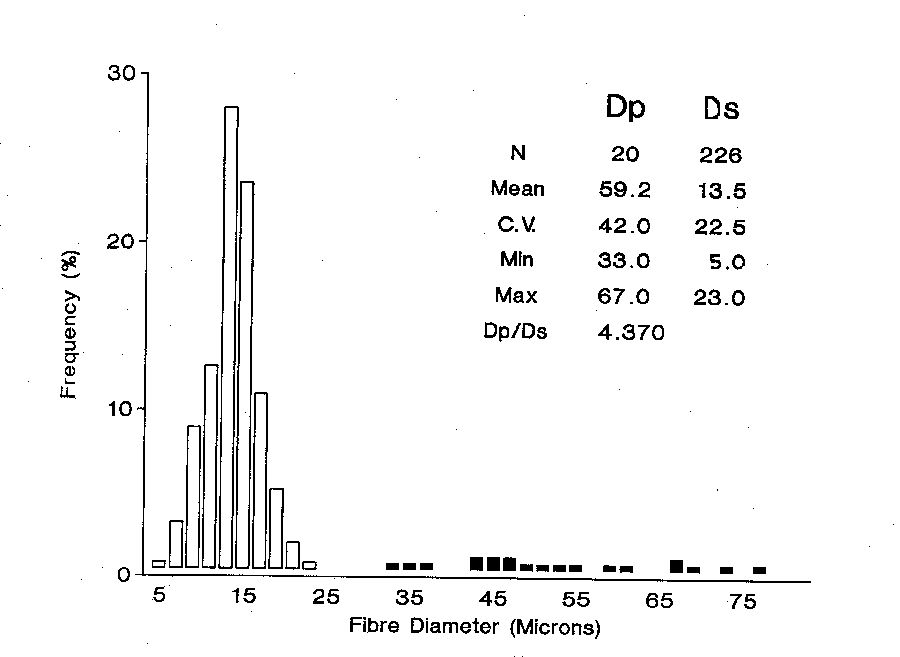
\includegraphics[width=\textwidth,trim = 0 0 0 120]{images/fig2.png}
  \caption{Fibre diameter histogram for the Barbary specimen of 
	   Figure~\ref{fig:1}.
	   Primary fibre frequencies are shown as shaded classes.}
  \label{fig:2}
\end{figure}

%\end{document}


%\documentclass{article}
%\usepackage{graphicx,subfigure}
%\begin{document}

\begin{figure}[tbp]
  \centering
  \includegraphics[width=\textwidth, trim = 0 0 0 20]{images/fig3.png}
  \caption{Transverse section of skin from a modern medium Australian Merino
        with no evidence of primitive characteristics, showing (a)
        primary fibres (20 $\mu m$) (b) secondary fibres (20 $\mu m$) .
        Plate (i) x ...... magnification.}
  \label{fig:3}
\end{figure}

%\end{document}

%\documentclass{article}
%\usepackage{graphicx,subfigure}
%\begin{document}

\begin{figure}[h]
  \centering
  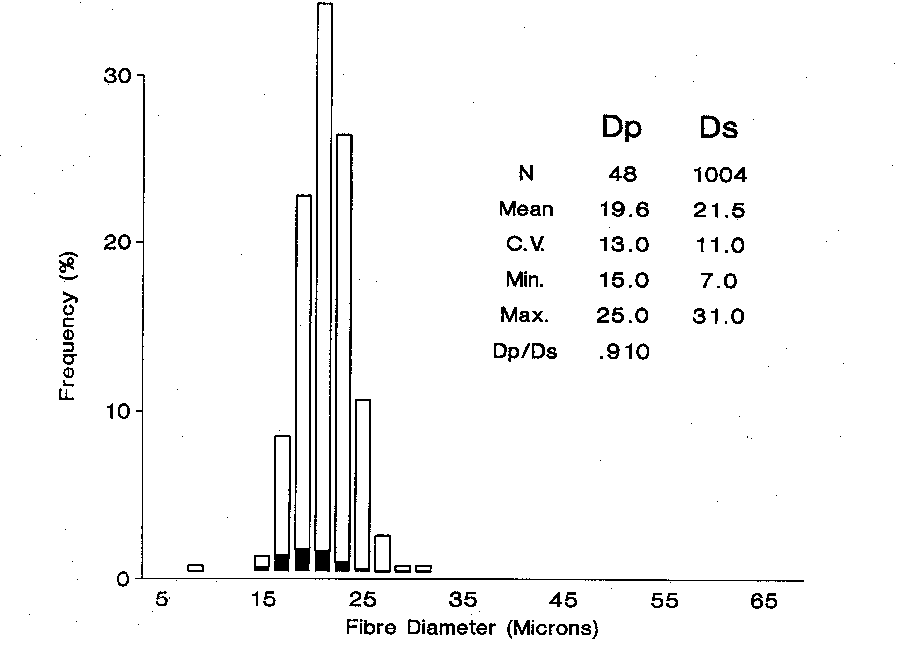
\includegraphics[width=\textwidth, trim = 0 0 0 120]{images/fig4.png}
  \caption{Fibre diameter histogram for the Merino specimen of
	   Figure~\ref{fig:3}.
	   Primary fibre frequencies are shown as shaded classes.}
  \label{fig:4}
\end{figure}

%\end{document}


    The most easily quantified characteristics in Table~\ref{tb:2} are average
diameter of primary and secondary fibres (Dp and Ds) and S/P ratio.  We
illustrate quantitative variation along the evolutionary series in Figures 5
and 6.  The position of British Longwool breeds in Figures 5 and 6 is of
interest in relation to their suspected role in evolution of some Australian
Merino strains. The Merinos are as close to the primitive Soay as they are to
the Longwools in Figures 5 and 6.

%\documentclass{article}
%\usepackage{graphicx,subfigure}
%\begin{document}

\begin{figure}[h]
  \centering
  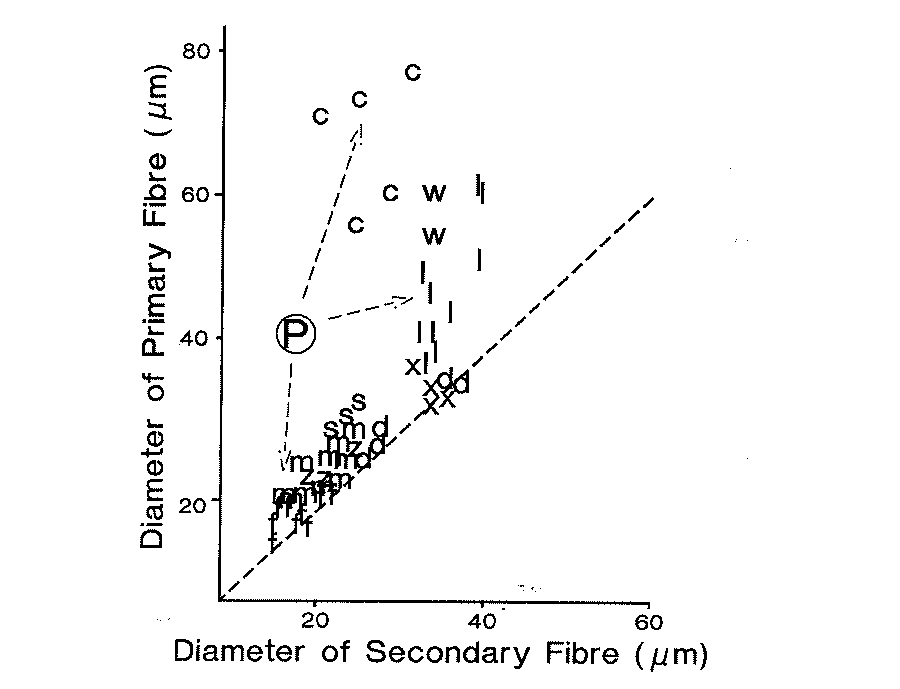
\includegraphics[width=1.3\textwidth, trim = 80 0 0 120]{images/fig5.png}
  \caption{   Relationship of primary fibre diameter (Dp) to secondary fibre
	      diameter (Ds) across a range of breeds.  Data from Carter (1968)
	  and CSIRO (unpublished).  Suggested lines of evolution of the
          major breeds shown $-\ -\ -\ -\ ->$.  $Dp/Ds$ ratio $ = 1$ 
	  shown $-\ -\ -\ -\ -\ -$. Letter codes denote breed;
f,  Fine Merino;
m,  Medium Merino;
s,  Strong Merino;
z,  Polwarth;
x,  Corriedale;
l,  Longwool;
d,  Downwool;
c,  Carpet Wool;
P,  Primitive;
w,  Wiltshire Horn. }
  \label{fig:5}
\end{figure}

%\end{document}

%\documentclass{article}
%\usepackage{graphicx,subfigure}
%\begin{document}

\begin{figure}[h]
  \centering
  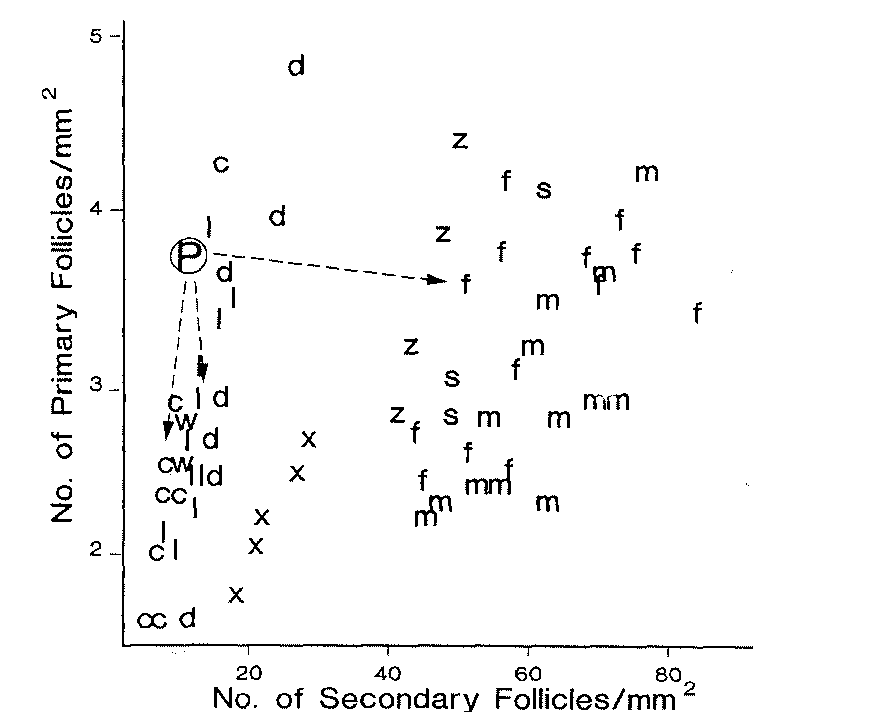
\includegraphics[width=1.3\textwidth, trim = 80 0 0 120]{images/fig6ri.png}
  \caption{ Relationship of primary fibre density (Np) to secondary fibre
      density (Ns) across a range of breeds.  Data from Carter (1968)
      and CSIRO unpublished.  Suggested lines of evolution of major
      breeds shown $-\ -\ -\ ->$. 
      Letter codes for breeds as in Figure~\ref{fig:5}.}
  \label{fig:6}
\end{figure}

%\end{document}


    Figure 7 illustrates changes in follicle group arrangement and fibre
medullation through four stages of Merino evolution described in Table~\ref{tb:2}. 
These changes are more difficult to quantify but are of value in visual
examination of skin sections.  The changes in follicle arrangement are
obviously a consequence of increased occurrence of compound secondary
follicles (Hardy and Lyne~\cite{hard:56}) as one moves down the evolutionary series. 
One cannot see compound follicles in a single transverse skin section, but
follicle arrangement reflects their presence.

%\documentclass{article}
%\usepackage{graphicx,subfigure}
%\begin{document}

\begin{figure}[h]
  \centering
  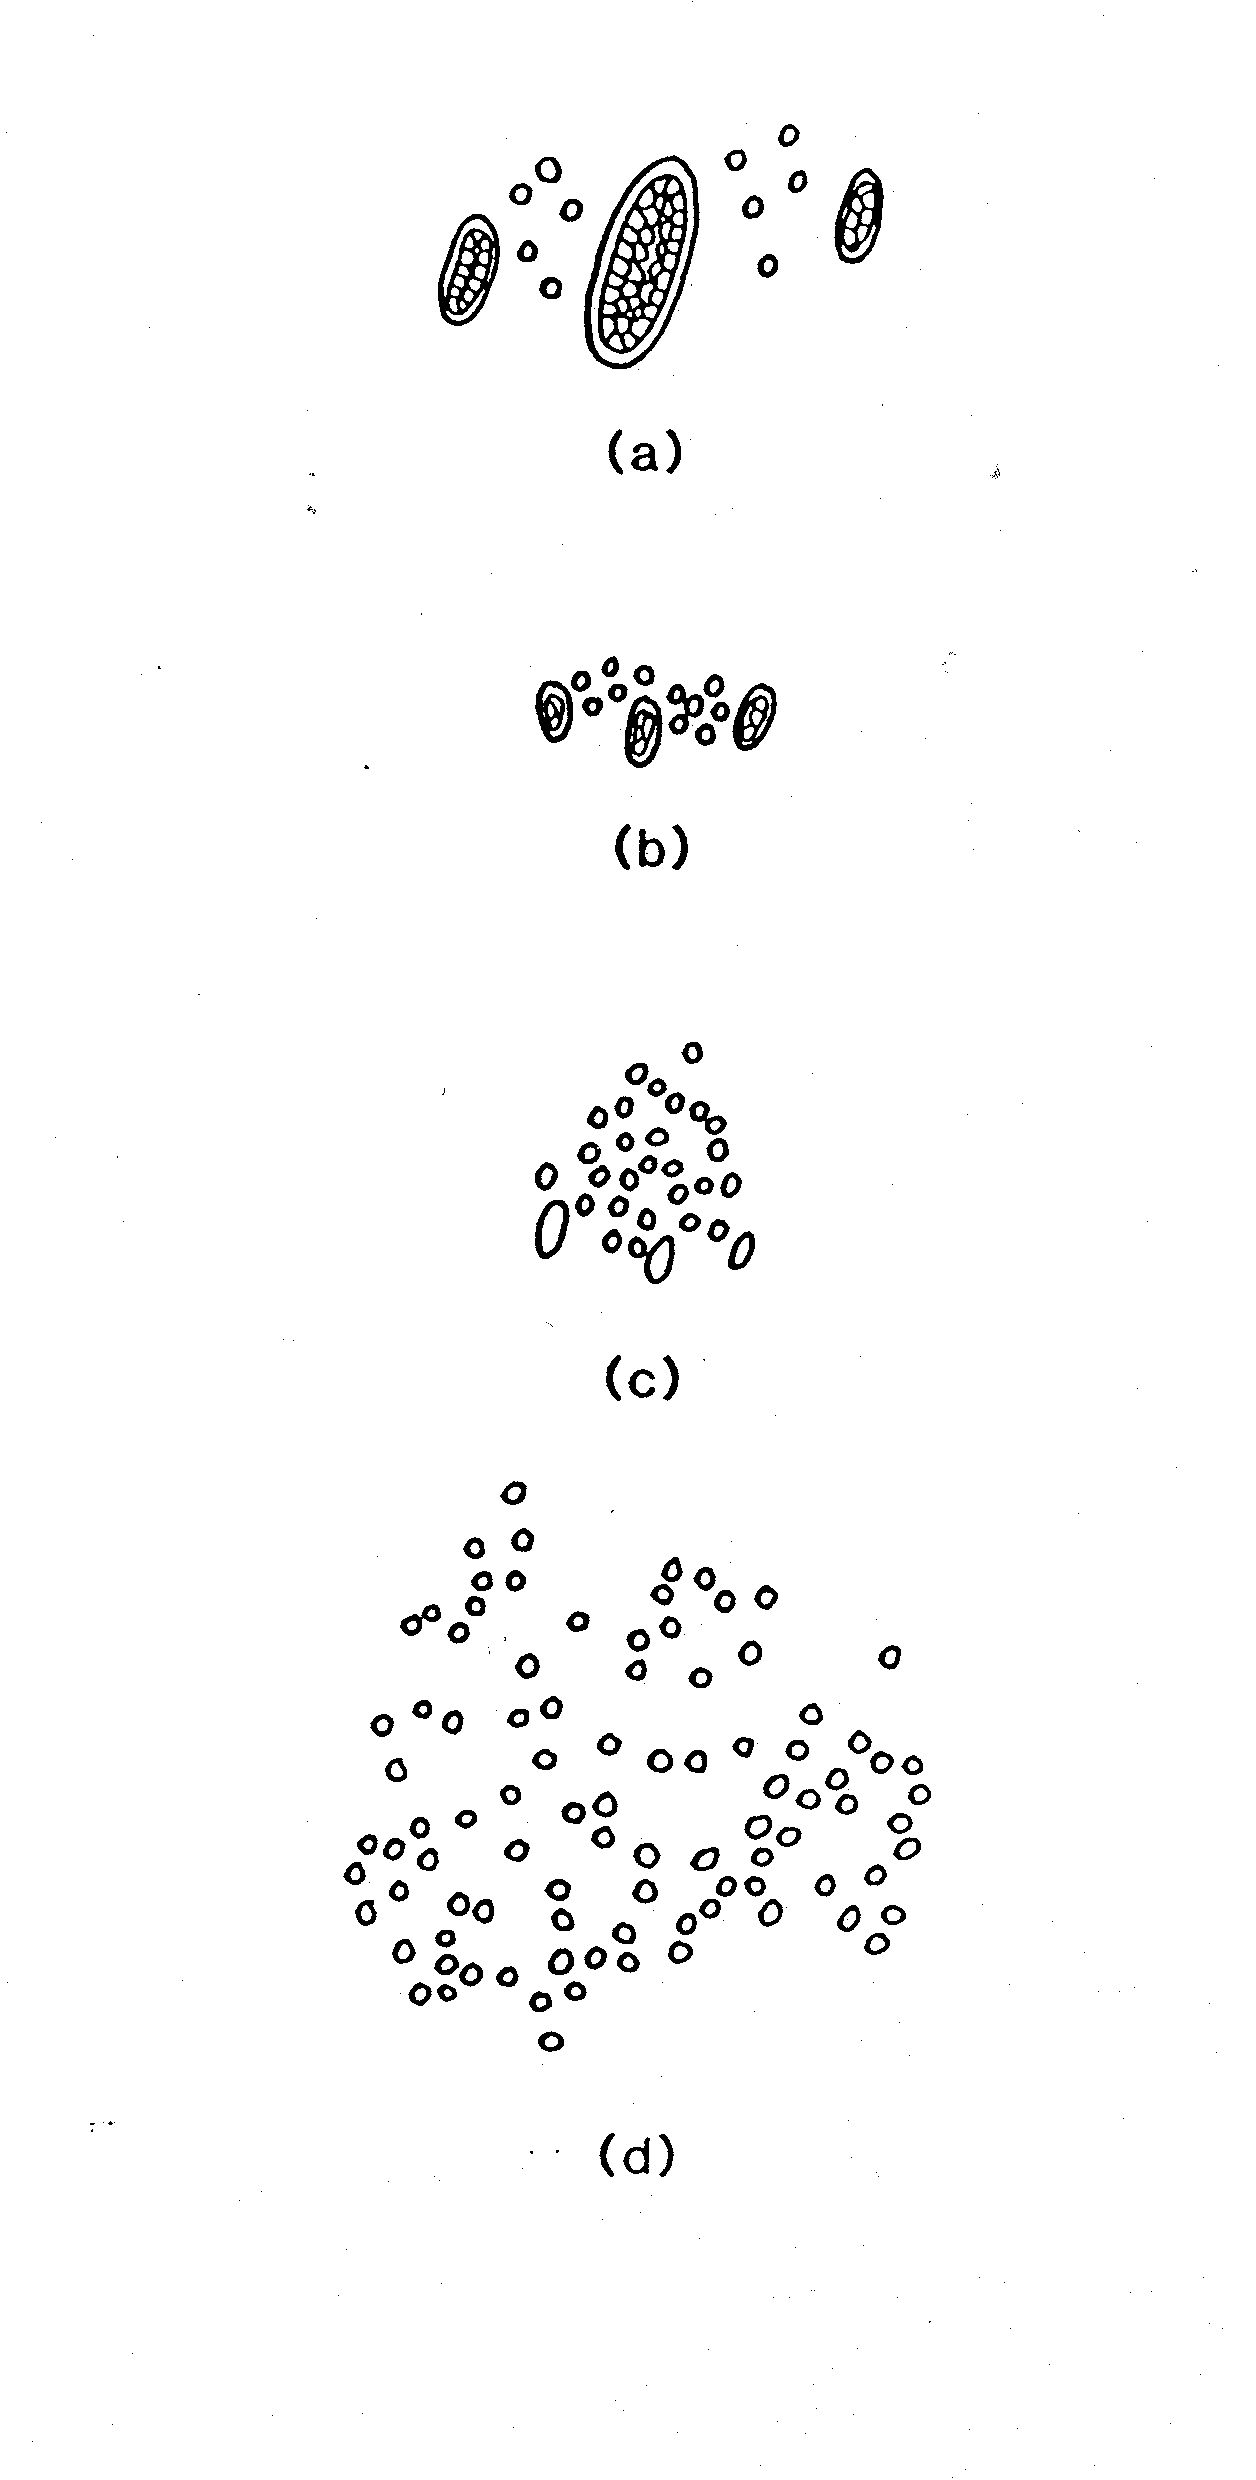
\includegraphics[width=0.8\textwidth, trim = 0 90 0 130]{images/fig7.png}
  \caption{ Tracings of fibre outlines showing changes in follicle group
    arrangement, fibre diameter and medullation through the four
    stages of Merino evolution described in Table 1.  (a) wild sheep,
    (b) primitive domestic sheep, (c) ancient fine/medium wool,
    (d) true fine wool.  Magnification x ....}
  \label{fig:7}
\end{figure}

%\end{document}


    Considerable caution needs to be applied in interpreting Dp and Ds data
from skin biopsy material, because fibres are sectioned at a single point in
their growth cycle.  If, for example, primary fibres are of a seasonal
shedding type, then the point at which they are cross-sectioned could be:-
\begin{itemize}
\item  a brush-end (unmedullated and coarse)
\item  a regrowth tip (unmedullated and fine)
\item  an actively growing fibre (medullated and coarse)
\end{itemize}
so that Dp and medullation data would depend on the season in which the sheep
was sampled.
    If, on the other hand, primary fibres were shedding asynchronously, then
a specimen taken at a given season might exhibit all three above possibilities
simultaneously, resulting in a very wide distribution of primary fibre
diameters, ranging from fine regrowth tips of less than 15 microns to heavily
medullated fibres of greater than 50 microns.
    Since skin characteristics are subject to environmental effects 
(Short~\cite{shor:58}),
it is not sound practice to sample sheep from one flock at one time and
to draw conclusions regarding the genetic merit of that flock, absolutely or
relative to other flocks.  However it is valid to compare animals within a
flock grazed under similar conditions, or to compare flocks in a common
environment.  These requirements cannot be strictly met across vast expanses
of time and space, so some of the material presented in this report depends
on an unverifiable assumption that the sheep sampled grazed under comparable
conditions.  Where possible we have taken steps to ensure this, by sampling
ewes rather than rams, by taking a random sample of sheep from a mob, by
avoiding drought or hand-fed conditions and by correcting for environmental
differences where these could be estimated.

\clearpage
\subsection{Incidence of Primitive Individuals in Industry Flocks}
    In the 1940's and early 1950's CSIRO sampled hogget ewes from a number
of leading Australian Merino studs.  Results have been summarized by Carter
and Clarke~\cite{cart:57a} and Carter~\cite{cart:68}. 
We have re-examined these data and are
representing it, in Table~\ref{tb:3}, to highlight individual variation in Dp/Ds ratio. 

%\documentclass{article}
%\usepackage{lscape}
%\begin{document}

\begin{landscape}
\begin{table}
\centering
\caption{Variation in Diameter of Primary and Secondary Fibres in Sheep from a Number of Leading Australian Merino Studs Sampled by CSIRO over the Period 1948-52. Data from Carter (unpubished and 1968).}
\label{tb:3}
\vspace{0.1in}
\begin{tabular}{l|r|rrr|rrr|r}  \hline
 Strain & Flock & \multicolumn{3}{c|}{Mean} &  \multicolumn{3}{c|}{Percent with Dp/Ds} &  Number \\ \cline{3-8}
        &       & Dp & Ds & Dp/Ds &   $>1.2$ &  $>1.5$ & $>1.8$ & Sampled \\ \hline

Early Fine Merino      &  1    &  $19.2\pm.34$   & $17.2\pm.19$  & $1.11\pm.021$  & 26.7  & 0.0  & 0.0  & 30 \\ \hline
 
Tas. Fine Merino       &  2    &  $18.4\pm.49$   & $17.8\pm.30$  & $1.03\pm.023$  &  9.5  & 0.0  & 0.0  & 21 \\
                       &  4    &  $19.2\pm.47$   & $16.2\pm.21$  & $1.15\pm.022$  & 36.4  & 0.0  & 0.0  & 22 \\
                       &  6    &  $19.3\pm.40$   & $16.7\pm.28$  & $1.15\pm.028$  & 33.3  & 0.0  & 0.0  & 21 \\
                       &  7    &  $19.9\pm.56$   & $18.8\pm.42$  & $1.02\pm.031$  &  8.7  & 0.0  & 0.0  & 23 \\
                       &  8    &  $20.6\pm.83$   & $18.1\pm.60$  & $1.15\pm.05 $  & 37.5  & 6.3  & 0.0  & 16 \\ \hline

Vic. Fine Merino       & 10    &  $20.2\pm.55$   & $18.0\pm.37$  & $1.12\pm.025$  & 28.6  & 0.0  & 0.0  & 21 \\
                       & 11    &  $18.3\pm.52$   & $15.9\pm.33$  & $1.16\pm.037$  & 27.3  & 0.0  & 0.0  & 11 \\
                       & 12    &  $15.8\pm.59$   & $15.7\pm.45$  & $1.01\pm.039$  &  7.7  & 0.0  & 0.0  & 13 \\
                       & 13    &  $22.7\pm.89$   & $19.9\pm.45$  & $1.15\pm.041$  & 38.1  & 4.8  & 0.0  & 21 \\ \hline

NSW Fine Merino        & 14    &  $19.0\pm.54$   & $17.1\pm.68$  & $1.13\pm.032$  & 19.0  & 0.0  & 0.0  & 21 \\ \hline

Non-Peppin Medium Merino &  15 &  $23.0\pm.50$   & $22.6\pm.42$  & $1.02+.026  $  & 6.0   & 0.0  & 0.0  & 25 \\
                       & 16    &  $22.3\pm.72$   & $21.0\pm.43$  & $1.07\pm.036$  & 22.7  & 0.0  & 0.0  & 22 \\
                       & 17    &  $26.6\pm.79$   & $22.3\pm.45$  & $1.20\pm.038$  & 38.1  & 9.5  & 0.0  & 21 \\ \hline

Peppin Medium Merino   & 18    &  $29.8\pm.96$   & $23.7\pm.28$  & $1.26\pm.038$  & 56.7  & 20.0 & 0.0  & 30 \\
                       & 19    &  $25.1\pm.97$   & $17.8\pm.53$  & $1.43\pm.53 $  & 80.0  & 25.0 & 15.0 & 20 \\
                       & 20    &  $28.0\pm.80$   & $22.8\pm.54$  & $1.23\pm.025$  & 60.0  & 0.0  & 0.0  & 20 \\
                       & 21    &  $25.7\pm.80$   & $23.2\pm.51$  & $1.11\pm.036$  & 30.0  & 0.0  & 0.0  & 20 \\
                       & 22    &  $21.6\pm.63$   & $17.1\pm.36$  & $1.27\pm.050$  & 42.9  & 19.0 & 4.8  & 21 \\
                       & 23    &  $25.5\pm1.14$ &  $19.9\pm.38$  & $1.25\pm.052$  & 66.7  & 13.3 & 0.0  & 15 \\
                       & 24    &  $21.1\pm1.21$ &  $16.8\pm.41$  & $1.27\pm.096$  & 54.5  & 9.1  & 9.9  & 11 \\
                       & 25    &  $22.5\pm.66$   & $19.2\pm.43$  & $1.18\pm.031$  & 38.1  & 0.0  & 0.0  & 21 \\ \hline

Strong Merino          & 26    &  $29.7\pm1.25$ &  $22.5\pm.42$  & $1.33\pm.061$  & 71.4  & 14.3 & 9.5  & 21 \\
                       & 27    &  $30.8\pm.78 $  & $23.7\pm.38$  & $1.30\pm.035$  & 76.2  & 19.0 & 0.0  & 21 \\
                       & 28    &  $32.6\pm1.11$ &  $24.7\pm.44$  & $1.33\pm.046$  & 66.7  & 14.3 & 4.8  & 21 \\ \hline

\end{tabular}
\end{table}
\end{landscape}

%\end{document}


If one arbitrarily regards sheep with $Dp/Ds > 1.5$ as showing primitive
characteristics then Table~\ref{tb:3} shows that they occur in all strains of Merino,
and in all environments, and that individual flocks vary in the frequency of
occurrence.
    Gallagher and Yeates~\cite{gall:70a}
studied the incidence of coarse fibres in
two Merino flocks of Tasmanian and Peppin origin.  They found percentages of
fibres exceeding 30 microns of 5.4, 4.7 and 11.5 at the neck, mid-side and
breech regions in flock 1, and 3.6, 3.9 and 10.0 respectively in flock 2. 
Corresponding percentages of medullated fibres were 0.17, 0.15 and 0.28% in
flock 1, and 0.11, 0.11 and 0.20% in flock 2.  It was noted in their
discussion that "one Merino ewe in flock 1 exhibited long coarse largely non-
medullated fibres projecting beyond the staple tip, a fleece characteristic
which Marston~\cite{mars:55} described as being reminiscent of the coarse outer and
fine inner coat of the primitive sheep".

    In a later paper Gallagher~\cite{gall:70}
surveyed 1014 bales of Merino wool,
finding a 1.1\% incidence of medullation (up to 3.3\% in individual lots) and
noting that this constituted an increase over estimates of previous workers. 
The average incidence of fibres over 30 microns in this survey was 2.4\%. 
Unfortunately figures for individual lots were not published.
    We have recently sampled sheep from a small number of today's leading
Merino studs.  Individual variation in Dp/Ds ratio is shown in Table~\ref{tb:4}. 
%\documentclass{article}
%\usepackage{lscape}
%\begin{document}

\begin{landscape}
\begin{table}
\centering
\caption{Variation in Diameter of Primary and Secondary Fibres in a Random Sample of 
         Ewes from a Number of Leading Merino Studs Sampled by CSIRO in 1987-88, 
	 and from two Studs and two Commercial Flocks Sampled by CSIRO in 1977.}
\label{tb:4}
\vspace{0.1in}

\begin{tabular}{l|r|rrr|rrr|r}  \hline
 Strain & Flock & \multicolumn{3}{c|}{Mean} &  \multicolumn{3}{c|}{Percent with Dp/Ds} &  Number \\ \cline{3-8}
        &       & Dp & Ds & Dp/Ds &   $>1.2$ &  $>1.5$ & $>1.8$ & Sampled \\ \hline

 Vic. Fine Merino       & 1     & $20.7\pm.31$   & $19.1\pm.24$   & $1.08\pm.014$  & 17.3  & 0.0  & 0.0  & 81 \\ \hline

 NSW Fine Merino        & 2     & $21.3\pm.45$   & $20.2\pm.34$  & $1.06\pm.015$  & 10.9  & 0.0  & 0.0  & 46 \\
                        & 3     & $20.3\pm.43$   & $20.1\pm.27$  & $1.02\pm.023$  &  6.25 & 0.0  & 0.0  & 32 \\ \hline

 Non-Peppin Medium Merino  &  4 & $21.1\pm.27$   & $19.0\pm.18$  &  $1.07\pm.014$ &  18.7 & 2.7  & 0.0  & 150 \\ \hline

 Peppin Medium Merino   & 5     & $27.6\pm.41$   & $24.6\pm.17$  & $1.13\pm.017$  & 26.0  & 5.0  & 0.0  & 100 \\
                        & 6     & $29.3\pm.46$   & $25.0\pm.28$  & $1.18\pm.019$  & 37.0  & 3.7  & 1.2  & 81 \\
                        & 7     & $24.0\pm.35$   & $22.5\pm.20$  & $1.07\pm.015$  & 18.3  & 0.0  & 0.0  & 60 \\
                        & 8     & $25.6\pm.47$   & $22.6\pm.21$  & $1.12\pm.021$  & 19.7  & 7.6  & 0.0  & 66 \\
                        & 9     & $24.4\pm.35$   & $20.7\pm.21$  & $1.18\pm.016$  & 32.9  & 1.3  & 0.0  & 76 \\ \hline

 Strong Merino          & 10    & $30.1\pm.39$  &  $23.8\pm.25$ &  $1.32\pm.022$ &  68.0 & 16.0 & 4.0  & 50 \\ \hline

 

\end{tabular}
\end{table}
\end{landscape}

%\end{document}


Animals showing a primitive Dp/Ds ratio continue to occur in our Merino
population, and the extent of the problem continues to vary between studs. 
There were no individuals with $Dp/Ds > 1.5$ in the fine-wool flocks sampled
this time.  Figures 8 and 9 show fibre diameter histogram and skin section of
a primitive individual from one of today's leading Australian Merino studs. 
It remains to be established whether there has been a significant change since
Carter's survey of the 1940's, but the phenomenon is certainly still visible. 
It would be of considerable interest to locate skin and fleece specimens
dating from before 1940, to obtain some indication as to whether recurrence
of the primitive type has always been a feature of the Merino.

%\documentclass{article}
%\usepackage{graphicx,subfigure}
%\begin{document}

\begin{figure}[h]
  \centering
  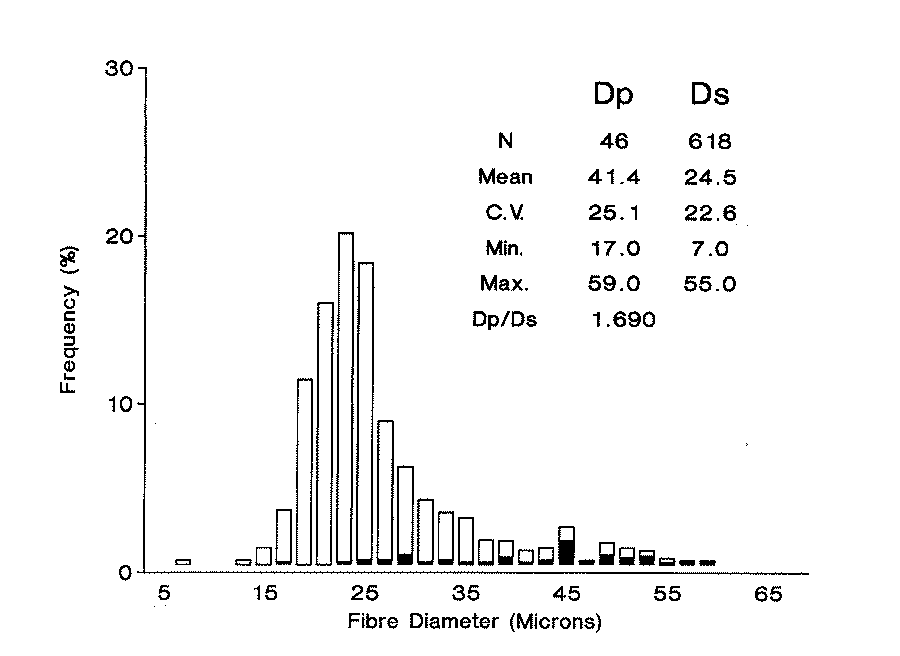
\includegraphics[width=\textwidth,trim = 0 0 0 20]{images/fig8.png}
  \caption{Fibre diameter histogram of a hogget ewe from a leading
     Australian Merino stud.  Note the high frequency of large primary
     and secondary fibres and the simultaneous presence of fine
     primary fibres.  The fine primaries are probably regrowth tips
     indicating shedding.}
  \label{fig:8}
\end{figure}

%\end{document}

%\documentclass{article}
%\usepackage{graphicx,subfigure,lscape}

%\newcommand{\goodgap}{%
%  \hspace{\subfigtopskip}%
%  \hspace{\subfigbottomskip}}

%\begin{document}

%\begin{landscape}
\begin{figure}[p]
  \centering
  \subfigure[Plate (i) x... magnification.]{
    \label{fig:9(i)}
    \includegraphics[width=0.65\textwidth, trim = 0 20 0 140]{images/fig9a.png}
  }
  \subfigure[Plate (ii) x... magnification.]{
    \label{fig:9(ii)}
    \includegraphics[width=0.65\textwidth, trim = 0 20 0 20]{images/fig9b.png}
  }
  \subfigure[Plate (iii) x... magnification.]{
    \label{fig:9(iii)}
    \includegraphics[width=0.65\textwidth, trim = 0 20 0 20]{images/fig9c.png}
  }
      \caption{ Transverse section of skin from the Australian Merino specimen
      of Figure~\ref{fig:8}.  Note (a) central primary follicle from which fibre
      has shed, (b) large lateral primary fibres (40 $\mu m$), (c) central
      primary fibre with fine fibre regrowth tip (78 $\mu m$), (d) wedge shaped
      arrangement of secondary follicles extending between the row of primary
      follicles, similar to the ancient fine/medium wool in Figure~\ref{fig:7}.}
  \label{fig:9}
\end{figure}

%\end{landscape}
%\end{document}


    Because industry flocks do not have experimental controls, one cannot
draw conclusions from the above observations as to why sheep showing primitive
characteristics occur.  One cannot even say whether the cause is genetic or
environmental.  We turn to research flocks for an indication of possible
causes.

\clearpage
\subsection{Incidence of Primitive Individuals in Research Station Flocks}
    Occurrence of animals showing primitive characteristics was first noted
in CSIRO selection experiment no. 32.  This experiment was designed to mimic
visual classing methods which place emphasis on skin thickness or "productive
skins" (Coy~\cite{coy:79}.
This experiment consisted of three lines selected for: 
increased follicle depth (Nay 1973) (line 1) increased number of follicles per
head (line 2), and simultaneous increase in follicle depth and follicle number
per head (line 3) over the period 1978-85.  The animals grazed with an
unselected control line.  Foundation animals for experiment 32 were CSIRO
experimental sheep upgraded by mating with rams from a Victorian fine Merino
stud.  Control line animals were of medium Peppin origin, thus providing an
environmental trend control, assuming that both strains would react equally
to environmental change.  Observations of distribution of diameter of primary
and secondary fibres were only available on the 1982-85 drop animals;  that
is for the years in which automated image analysis was employed. 
Table~\ref{tb:5} summarizes performance of 1982-85 drop animals. 

%\documentclass{article}
%\usepackage{lscape}
%\begin{document}

\begin{landscape}
\begin{table}
\centering
\caption{Variation in Diameter of Primary and Secondary Fibres of 1982-85 Drop
         Animals in CSIRO Experiment No. 32.
	 (Means obtained as drop x line effects in a linear model adjusting
	  for sex and age of dam)}
\label{tb:5}
\vspace{0.1in}

\begin{tabular}{l|r|rrr|rrr|r}  \hline
 Line & Drop & \multicolumn{3}{c|}{Mean} &  \multicolumn{3}{c|}{Percent with Dp/Ds} &  Number \\ \cline{3-8}
        &       & Dp & Ds & Dp/Ds &   $>1.2$ &  $>1.5$ & $>1.8$ & Sampled \\ \hline


High follicle depth   & 1982   & $24.4\pm.74$  & $21.1\pm.42$  & $1.16\pm.037$  & 38.5  & 4.6  & 0.0 &  65 \\
                      & 1983   & $21.9\pm1.08$ & $20.1\pm.62$  & $1.09\pm.054$  & 10.9  & 2.2  & 0.0 &  46 \\
                      & 1984   & $25.7\pm.84$  & $23.3\pm.48$  & $1.10\pm.041$  & 19.4  & 0.0  & 0.0 &  36 \\
                      & 1985   & $25.7\pm.72$  & $20.5\pm.41$  & $1.26\pm.036$  & 61.5  & 11.5 & 0.0 &  91 \\ \hline

High follicle number  & 1982   & $21.9\pm.72$  & $20.0\pm.41$  & $1.09\pm.036$  & 26.7  & 3.3  & 0.0 &  90 \\
                      & 1983   & $20.6\pm.90$  & $20.1\pm.51$  & $1.03\pm.044$  & 14.3  & 2.9  & 0.0 &  35 \\
                      & 1984   & $22.4\pm1.12$ & $21.5\pm.64$  & $1.05\pm.055$  &  0.0  & 0.0  & 0.0 &  34 \\
                      & 1985   & $22.0\pm.79$  & $19.8\pm.45$  & $1.12\pm.039$  & 19.1  & 2.9  & 0.0 &  68 \\ \hline

High depth and number & 1982   & $25.0\pm.77$  & $20.5\pm.44$  & $1.23\pm.039$  & 53.7  & 14.6 & 1.2 &  82 \\
                      & 1983   & $26.1\pm.65$  & $19.5\pm.52$  & $1.16\pm.045$  & 30.8  & 0.0  & 0.0 &  39 \\
                      & 1984   & $24.6\pm.86$  & $20.8\pm.49$  & $1.18\pm.043$  & 37.5  & 3.6  & 0.0 &  56 \\
                      & 1985   & $25.2\pm.72$  & $20.0\pm.41$  & $1.27\pm.036$  & 62.5  & 11.4 & 2.3 &  88 \\ \hline

Unselected control    & 1982   &            &           &            &       &      &     &     \\
                      & 1983   &  $26.1\pm.65$ & $21.9\pm.38$  & $1.20\pm.032$ &  44.7 &  4.3 & 0.0 &  47 \\
                      & 1984   &            &           &            &       &      &     &     \\
                      & 1985   &  $25.4\pm.60$ & $22.1\pm.34$  & $1.15\pm.029$ &  27.1 &  6.3 & 0.0 &  48 \\ \hline
  
\end{tabular}
\end{table}
\end{landscape}

%\end{document}


One would not expect to be
able to detect a trend over these four years;  one can only compare lines at
this point in time.  The result of greatest relevance here is the higher
frequency of animals with high Dp/Ds ratios in lines 1 and 3, particularly in
the 1985 drop.  In a closely controlled experiment of this nature, one can
conclude that the higher  frequency of primitive animals was caused by
selection for increased follicle depth.  While the change in line average
Dp/Ds is not large, some very extreme individuals (with Dp halfway between a
fine Merino and a primitive Soay) were produced.  One of these is illustrated
in Figures 10 and 11.

%\documentclass{article}
%\usepackage{graphicx,subfigure}
%\begin{document}

\begin{figure}[h]
  \centering
  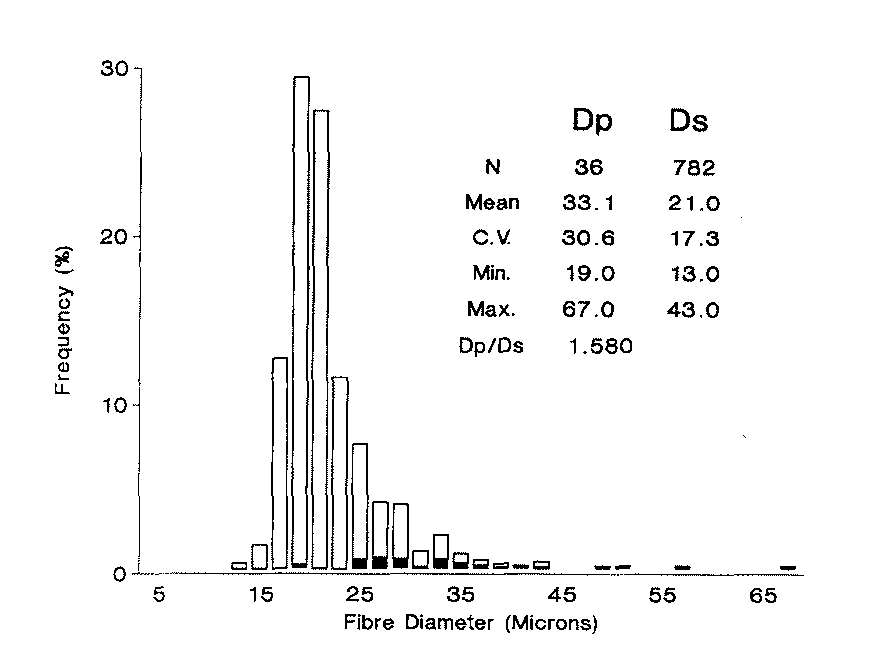
\includegraphics[width=\textwidth,trim = 0 0 0 20]{images/fig10ri.png}
  \caption{Fibre diameter histogram of a 1985 drop hogget ewe from the high
      follicle depth selection line of CSIRO experiment No. 32.  In
      this case most of the large fibres are primaries.}

  \label{fig:10}
\end{figure}

%\end{document}

%\documentclass{article}
%\usepackage{graphicx,subfigure}
%\begin{document}

\begin{figure}[h]
  \centering
  \includegraphics[width=\textwidth, trim = 0 0 0 20]{images/fig11.png}
  \caption{Transverse section of skin from the specimen of 
      Figure~\ref{fig:10}.  Note
      (a) large medullated central primary fibre and (b) large non-
      medullated lateral primary fibre.
      Plate (i) x... magnification.}
  \label{fig:11}
\end{figure}

%\end{document}


    We have one further piece of evidence from experiment 32.  If primary
fibres are coarser in the adult fleece, one would expect a correlated increase
in {\em hairiness} of the lamb birthcoat (Schinckel~\cite{schi:58}.
Figure 12 shows that
there has been an increase in birthcoat score in lines 1 and 3 of experiment
32.  These data are particularly valuable as they span the whole period of
selection, and show that the changes referred to have only become obvious in
the last few drops.

%\documentclass{article}
%\usepackage{graphicx,subfigure}
%\begin{document}

\begin{figure}[h]
  \centering
  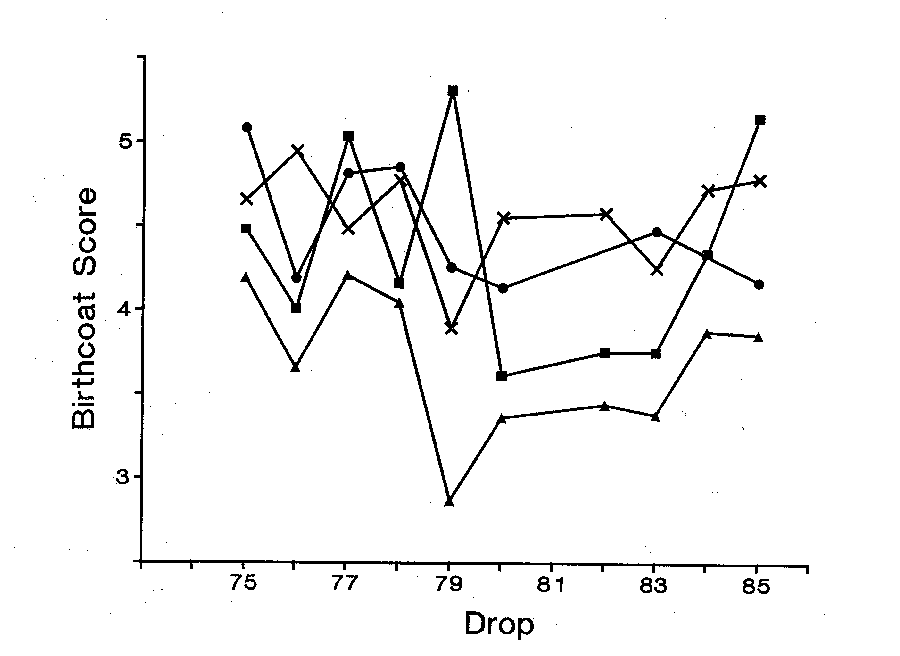
\includegraphics[width=\textwidth,trim = 0 0 0 120]{images/fig12.png}
  \caption{Average birthcoat scores of successive drops in CSIRO experiment
      32. $\blacksquare---\blacksquare$ line 1;  $\blacktriangle---\blacktriangle$ line 2; $X-----X$
      line 3;  $\bullet---\bullet$  unselected control line.}
  \label{fig:12}
\end{figure}

%\end{document}


    If a mere 8 years of selection could expose this amount of variation in
primitive characteristics, one is led to ask whether other selection regimes
could do better (or worse depending on one's point of view)?  This led us to
ask whether primitive sheep could be found in industry flocks.  Data already
presented show that primitive sheep are not peculiar to research flocks - they
occur throughout the Australian Merino industry in all strains.
    We looked also at CSIRO selection experiment no. 10 selection for high
clean wool weight with no culling to prevent increase in average fibre
diameter), over the period 1958-88. 
Table~\ref{tb:6} summarizes performance of 1979 and 1982 drop animals. 

%\documentclass{article}
%\usepackage{lscape}
%\begin{document}

\begin{landscape}
\begin{table} 
\centering
\caption{Variation in Diameter of Primary and Secondary Fibres in Sheep from
         CSIRO Experiments No. 10 (high clean wool weight) and No. 1 (high
	 clean wool weight with average diameter and wrinkle held constant)}
\label{tb:6} 
\vspace{0.1in}

\begin{tabular}{l|r|rrr|rrr|r}  \hline
 Drop & Flock & \multicolumn{3}{c|}{Mean} &  \multicolumn{3}{c|}{Percent with Dp/Ds} &  Number \\ \cline{3-8}
        &       & Dp & Ds & Dp/Ds &   $>1.2$ &  $>1.5$ & $>1.8$ & Sampled \\ \hline

  1979   & expt 1  & $28.4\pm .82$  & $23.1\pm.30$  & $1.23\pm.037$  & 60.0 &   0.0  &  0.0 & 10 \\
  
         & expt 10 & $35.5\pm1.15$  & $15.1\pm.47$  & $1.41\pm.076$  & 40.0 &   20.0 & 10.0 & 10 \\
  
         & control & $26.5\pm .96$  & $21.2\pm.44$  & $1.25\pm.045$  & 50.0 &   10.0 &  0.0 & 10 \\ \hline
 
  
   1982  & expt 10 & $31.7\pm .45$  & $26.6\pm.26$  & $1.21\pm.020$  & 39.8 &   5.7  &  0.0 & 88 \\
  
         & control &     -      &     -     &     -      &   -  &   -    &  -   & - \\ \hline
\end{tabular}
\end{table}
\end{landscape}

%\end{document}


Figures 13 and 14 show one extreme individual.  These
animals are different from experiment 32.  In experiment 10 the entire fibre
diameter distribution has become coarse, not just the primary fibres.  The
animals in experiment 10 resemble British Longwools more than primitive two-
coated sheep.  This may be a reflection of their different origin;  foundation
animals in experiment 10 were Medium Peppin Merino, or of the different
selection regime.

%\documentclass{article}
%\usepackage{graphicx,subfigure}
%\begin{document}

\begin{figure}[h]
  \centering
  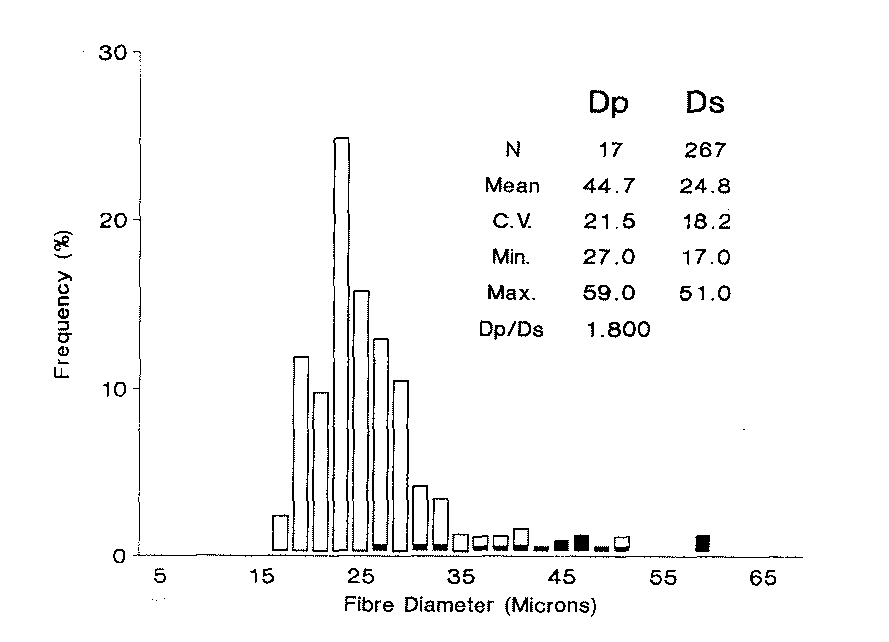
\includegraphics[width=\textwidth,trim = 0 0 0 20]{images/fig13ri.png}
  \caption{Fibre diameter histogram of a 198? drop hogget ewe from CSIRO
      experiment No. 10.  Note the high frequency of large primary and
      secondary fibres.}
  \label{fig:13}
\end{figure}

%\end{document}

%\documentclass{article}
%\usepackage{graphicx,subfigure}
%\begin{document}

\begin{figure}[h]
  \centering
  \subfigure[Plate (i) x... magnification.]{
    \label{fig:14(i)}
    \includegraphics[width=\textwidth, trim = 0 20 0 120]{images/fig14a.png}
  }
  \subfigure[Plate (ii) x... magnification.]{
    \label{fig:14(ii)}
    \includegraphics[width=\textwidth, trim = 0 20 0 20]{images/fig14b.png}
  }
  \caption{ Transverse section of skin from the specimen of 
	 Figure~\ref{fig:13}.  Plate
         (i) shows a trio group with large primary and secondary fibres.
	  Plate (ii) shows (a) a shed primary follicle, and (b) all
          unlabelled arrows show secondary follicles in various stages of
	  shedding. }
  \label{fig:14}
\end{figure}

%\end{document}


    We would also like to have looked at CSIRO selection experiment no. 1
-selected for high clean wool weight, with culling to prevent increase in
average fibre diameter or wrinkle.  Unfortunately, this experiment was
abandoned in 1977 and there are few surviving skin specimens.  There were some
primitive characteristics shown in 6 of 10 surviving specimens
(Table~\ref{tb:6}).  An
individual with $Dp/Ds = 1.4$ is illustrated in Figure 15.

%\documentclass{article}
%\usepackage{graphicx,subfigure}
%\begin{document}

\begin{figure}[h]
  \centering
  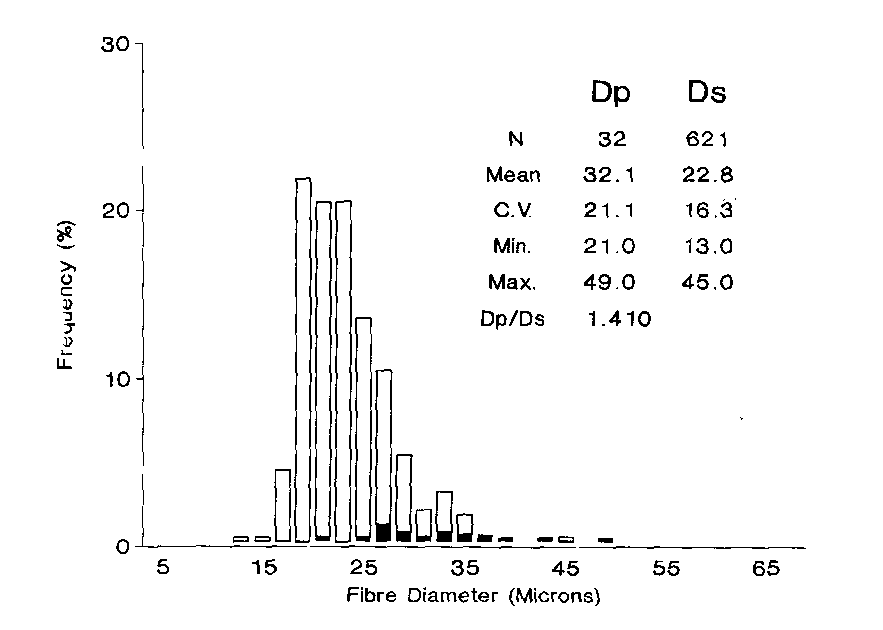
\includegraphics[width=\textwidth,trim = 0 0 0 120]{images/fig15ri.png}
  \caption{ Fibre diameter histogram of a 1976 drop hogget ewe from CSIRO
      experiment No. 1.  Note that the frequency of large primary and
      secondary fibres is not as large as in Figure~\ref{fig:13},
      but is higher than in Figure~\ref{fig:4}.}
  \label{fig:15}
\end{figure}

%\end{document}


    Barlow~\cite{barl:74}
published mean values of Dp and Ds for three drops of ewes
in high and low clean fleece weight and random flocks at NSWDA, Trangie, NSW. 
These data are summarised in Table~\ref{tb:7}.

%\documentclass{article}
%\begin{document}

\begin{table}[h]
\centering
\caption{Variation in Diameter of Primary and Secondary Fibres in three Drops
	 of Ewes from Trangie High and Low Fleece Weight and Random Flocks.}
%	 After Barlow~\cite{barl:74}.}
 \label{tb:7} 
\vspace{0.1in}

\begin{tabular}{l|r|rrr}  \hline
 Flock & Drop & \multicolumn{3}{c}{Mean}  \\ \cline{3-5}
        &       & Dp & Ds & Dp/Ds \\ \hline

  
  Fleece plus      & 1962    &  29.6   &  19.4    &  1.53 \\
  
                   & 1963    &  29.6   &  20.6    &  1.44 \\
  
                   & 1964    &  28.1   &  20.9    &  1.34 \\ \hline
  
  
   Random          & 1962    &  27.1   &  18.6    &  1.46 \\
  
                   & 1963    &  28.8   &  21.2    &  1.36 \\
  
                   & 1964    &  26.3   &  20.5    &  1.28 \\ \hline
  
  
   Fleece minus    & 1962    &  24.7   &  19.7    &  1.25 \\
  
                   & 1963    &  27.2   &  22.2    &  1.23 \\
  
                   & 1964    &  22.8   &  20.4    &  1.12 \\ \hline
\end{tabular}
% \caption{After Barlow~\cite[]{barl:74}}
\end{table}

%\end{document}


All three flocks exhibit higher Dp/Ds
ratios than the average industry medium Peppin flock in 
Tables~\ref{tb:3}~or~\ref{tb:4}, and
similar Dp/Ds ratios to the CSIRO research flocks in Table~\ref{tb:6}.
There is also
an obvious effect of selection - the highest Dp/Ds ratio in each drop occurred
in the Fleece Plus group.
    From the above observations on research flocks we can conclude that the
occurrence of sheep showing primitive characteristics has a genetic basis. 
It is not clear which types of artificial selection criteria will lead to
increased frequency of primitive characteristics, and it is not clear whether
natural selection or non-additive gene action are involved.  It is also
obvious, from Table~\ref{tb:5}, that characteristics such as Dp/Ds are influenced by
environment as well as inheritance, so that one has to be wary of drawing
conclusions from uncontrolled observations on a single flock.  There does seem
to be a general trend for research flocks, particularly random-bred flocks,
to display more extreme primitive characteristics than industry flocks of the
same strain.   We turn to more precise studies of quantitative variation for
a prediction of what is likely to occur under particular breeding objectives.

\clearpage
\subsection{Evidence of Primitive Trends from Genetic Parameter Estimates}
    Additive genetic parameters can be used to predict rate of change in a
population mean for a quantitative trait, under any artificial (i.e. man-
applied) selection method.  They cannot predict changes in mean due to natural
selection, or to non-additive gene action.  They also cannot alone predict
changes in population variability.
    We have obtained estimates of parameters needed to predict genetic
change in Dp and Ds from an analysis of variation between and within sire
families, using all of CSIRO's currently available data which amount to 793
progeny from 90 sire families.  These are summarized in Table~\ref{tb:8}.

%\documentclass{article}
%\usepackage{lscape}
%\begin{document}

\begin{landscape}
\begin{table} 
\footnotesize
\centering
\caption{Parameter Estimates and Standard Errors for Dp and Associated Traits
	 for Hogget Rams and Ewes Born in CSIRO Experiments 20 and 32.}
\label{tb:8} 
\vspace{0.1in}

\begin{tabular}{l|rrrrrrrrrr|}  \hline
   & Dp & Ds & Dp/Ds & CWW & FD & BW & dNLW & Follicle & Follicle & Birthcoat \\
   &    &    &       &     &    &    &      & Depth    & Number   & Score  \\ \hline

Mean & 23.9 & 20.6 &  1.17  &  2.5  & 18.5  &  35.4  & 1.34  & - &  73.5  &  3.6 \\

Phenotypic standard deviation &  3.9 & 2.2  & 0.18 &  0.58 & 1.6  &  6.9  & 0.47 &  - & 17.1 &  1.6 \\

Heritability   & $.64\pm.15$ & $.62\pm.14$ & $.73\pm.15$  & $.34\pm.11$  & $.96\pm.16$  & $.29\pm.11$ & $.18\pm.10$  & $.35$   & $.41\pm.12$  & $1.15\pm.16$ \\ \hline

Genetic correlation with: & & & & & & & & & & \\
    Ds               & $.29\pm.17$ & & & & & & & & &\\
    Dp/Ds            & $.80\pm.07$ & $-.35\pm.19$ & & & & & & & & \\
    CWW              & $.16\pm.22$ &  $.66\pm.18$ & $-.25\pm.22$ & & & & & & & \\
    FD               & $.40\pm.15$ & $.95\pm.05$  & $-.23\pm.17$ & $.82\pm.14$ & & & & & & \\
    BW             &  $-.35\pm.24$ & $.04\pm.24$  & $-.37\pm.24$ & $.35\pm.16$ & & & & & & \\
    dNLW             & $.52\pm.25$ & $.34\pm.28$  &  $.32\pm.26$ & $.52\pm.38$ & $.24\pm.25$ &  $-.22\pm.38$ & & & & \\
  Follicle depth     &     -     &    -       &  -         & -         & -         & -  & & & & \\
  Follicle number    & $-.32\pm.22$ &  $-.86\pm.24$  &  $.23\pm.20$ & $-.44\pm.23$ &  $-.77\pm.22$ &  $-.05\pm.27$ & $-3.7\pm.34$  &  - & & \\
  Birthcoat score & $.71\pm.01$   &  $-.03\pm.17$    &  $.70\pm.09$ & $-.16\pm.20$ & $.09\pm.15$   & $-.36\pm.21$  &  $.28\pm.25$  &   -  &  $-.11\pm.19$ &  \\ \hline

Phenotypic correlation with: & & & & & & & & & & \\
    Ds            &   $.39\pm.03$ & & & & & & & & & \\
    Dp/Ds         &   $.77\pm.02$ & $-.28\pm.04$ & & & & & & & & \\
    CWW           &   $.08\pm.04$ & $.22\pm.04$  & $-.08\pm.04$ & & & & & & &\\
    FD            &   $.40\pm.03$ & $.62\pm.03$  & $-.02\pm.04$ & $.32\pm.04$ & & & & & & \\
    BW            &  $-.04\pm.04$ & $.16\pm.04$  & $-.15\pm.03$ & $.17\pm.04$ & & & & & & \\
    dNLW          &   $.20\pm.04$ & $.08\pm.04$  & $.16\pm.04$  & $.19\pm.04$ & $.14\pm.04$ &  $-.23\pm.04$  & & & &\\
    Follicle depth \footnotemark[1] &   .16  &  .19   &   .06  &   .20  &    .00  &    .16   &   - & & & \\
    Follicle number &  $-.23\pm.0$4 & $-.44\pm.03$ &   $.06\pm.04$ & $.14\pm.04$  & $-.51\pm.03$  &  $.21\pm.04$ & $-.17\pm.04$ & $.03$ & &  \\
    Birthcoat score & $.37\pm.03$ & $-.02\pm.04$  &    $.50\pm.03$ & $.01\pm.04$  & $.13\pm.04$   & $-.04\pm.04$ & $-.03\pm.04$    & -  &  $-.03\pm.04$ & \\ \hline

\end{tabular}
\vspace{0.1in}
\footnotetext[1]{Preliminary estimates only, data incomplete.}
\normalsize
\end{table}
\end{landscape}

%\end{document}


These
parameters should be used with caution for two reasons:
\begin{itemize}
\item  some of the sires were not chosen at random,
\item  one needs about twice the data available to achieve acceptable standard
         errors, particularly for genetic correlations.
\end{itemize}
    However, there is reason for some confidence in the estimates of
Table~\ref{tb:8} because:
\begin{itemize}
\item  heritability of CWW,BW,dNLW agree closely with other published
    estimates.  Heritability of FD is high compared with estimates of Brown
    and Turner (1968) and Morley (1955) but the Armidale environment is
    known to differ in heritability of diameter and traits associated with
    it (Watson et al., 1977),
\item   genetic and phenotypic correlations among CWW,FD,BW,dNLW agree, at
         least in sign, with other published estimates.
\end{itemize}
    The most obvious result in Table~\ref{tb:8} is that traits Dp, Ds and Dp/Ds are
all highly heritable.  If fleece hairiness due to a high Dp were a problem in
any flock, one should be able to breed it out quite rapidly.  The fact that
hairiness is not so easily controlled in practise (several breeders have
commented to the authors that many years of visual selection against fleece
hairiness has not removed it from their flocks) suggests that there are forces
operating in Merino flocks which tend to favour recurrence of primitive hairy
sheep.  These forces could be:
\begin{itemize}
\item  natural selection may favour sheep with a high Dp, either through
    greater survival rates, enhanced reproduction rates, or better maternal
    ability,
\item   artificial selection (whether by classing or objective measurement) may
         favour sheep with a high Dp as a correlated response due to genetic
         correlation between Dp and the trait(s) selected.  This may be what has
         occurred in the various selection experiments discussed in the previous
         section;  however, the above results could also be explained if the
         selection applied did not oppose natural selection for high Dp,
\item    non-additive gene action may lead to reversion toward the
         {\em wild type}
         of fleece when artificial selection is relaxed.  This may be a factor
         explaining occurrence of primitive sheep in various industry flocks, as
         selection in industry flocks is not concentrated on a small number of
         traits as is the case in selection experiments,
\item    changes in degree of heterozygosis, through inbreeding or outcrossing
         may favour sheep with a high Dp, if Dp is correlated with fitness.  The
         magnitude of the genetic correlation between Dp and dNLW would suggest
         that this is a possibility.  This hypothesis would explain occurrence
         of primitive sheep in industry flocks which have recently crossed
         strains.  It may also explain the general high incidence of primitive
         sheep in Australian Merino flocks, as the large Australian flocks would
         have a lower rate of inbreeding than their original Spanish Merino
         ancestors.
\item Segregation of a single recessive gene with low frequency.  This
    possibility is considered unlikely because animal-to-animal
    distributions of Dp are continuous, with no trace of bimodality.
\end{itemize}

    One cannot distinguish between these possibilities from present data. 
In the discussion we consider the type of experiments needed to resolve these
issues.
    The second important result from Table~\ref{tb:8} is that Dp and Ds are under
somewhat separate genetic control, as evidenced by a 0.2 genetic correlation
between them, and differing genetic correlations with the other traits.  For
example CWW has a low positive correlation with Dp, but has a high positive
correlation with Ds.  Thus, from a genetic point of view, the fleece consists
of two partly independent fibre populations, and it is not surprising that
they occasionally respond independently in selection experiments and in
commercial flocks, as reported above.
    The third result from Table~\ref{tb:8} is obtained by placing an evolutionary
interpretation on the correlations.  If Dp/Ds is an index of {\em degree of
primitiveness} then the correlations imply that primitive sheep have a lower
CWW, higher Dp, lower Ds, lower BW, and higher dNLW, than the modern Merino. 
All of these inferences make sense at a breed comparison level.  Compared with
a primitive Soay the Merino is larger, less fit reproductively, and has a more
uniform fleece of greater weight.  It is well known that within-flock genetic
parameters are not necessarily the same as between breed genetic parameters; 
but they may be if they reflect strongly buffered developmental processes. 
The development of primary follicles is common to all animals with warm-
blooded metabolism - eutherian mammals, marsupials, monotremes, and debatably
birds (Carter~\cite{cart:65};  Rawles~\cite{rawl:65}). 
It is not surprising that such an
ancient developmental process would be strongly buffered by many generations
of selection of modifying genes, and would be strongly correlated with fitness
(Note high genetic correlation of Dp with dNLW) - we interpret this 
correlation as a reflection of a developmental link between follicle
development and homeothermy, temperature regulation being a well known factor
affecting fertility (Brown and Hutchinson~\cite{brow:73}).
    The final result from Table~\ref{tb:8} is that the genetic correlation between
Dp and total follicle number is negative.  Note that the only experimental
flock in which we have not noted an incidence of primitive sheep is the high
total follicle number line (line 2) of CSIRO experiment no. 32 reported above. 
We believe this reflects a developmental cause and effect relationship, for
which there is evidence from other CSIRO studies of the developmental process
of follicle formation, outlined below.

\clearpage
\subsection{Evidence from Developmental Studies of the Importance of Size of 
 Primary Follicles in Evolution of Merinos}
    CSIRO has undertaken extensive studies of prenatal follicle development
in Merino sheep (e.g. Hardy and Lyne~\cite{hard:56};  Moore~\cite{moor:84};
Moore and Jackson~\cite{moor:84a};  Moore et al.~\cite{moor:89}. 
Three types of follicles are initiated in the
foetus:  primary (P), secondary original (SO) and secondary derived (SD)
follicles.  These begin to appear in midside skin at about 60, 85 and 100 days
of gestation, respectively.  P and SO follicles form at separate initiation
sites, but SD follicles, which are the last to appear, develop as branches
from SO and other SD follicles and perhaps from P follicles also 
(Lyne~\cite{lyne:57}). 
The Merino sheep has a greater proportion of SO + SD follicles than any other
breed.
    Recent work supports a new hypothesis explaining follicle and fibre
formation in the developing foetus in a different way from the competition
hypothesis of Fraser and Short~\cite{fras:60}.
This has been alluded to in Moore et al.~\cite{moor:89} 
and is based on observations of (1) the relationships between
the dermal papilla component of the wool follicle and the productive
activities of the follicle, (2) the effects of single character selection on
the distribution of the three follicle types in the skin of the Merino and (3)
the effects of such selection on wool weight and its components.
    The dermal papilla of each follicle arises during foetal life and is
first recognisable as an aggregate of cells, adjacent to an epidermal
condensation, formed by migration of fibroblastic cells within the surrounding
mesenchyme.   These cells remain associated with the growing epidermal plug
during development and eventually become incorporated into a pocket at the
base of the mature follicle.  Unlike the follicle epithelium, proliferation
of papilla cells is low during development and absent in the mature follicle,
suggesting that absolute size of the papilla cell population may be determined
early during follicle development.  The close physical association maintained
between the papilla and epithelial components of the follicle, during periods
of active fibre growth, indicate a functional relationship.  Morphometric,
genetic and transplantation studies have confirmed that presence of a papilla
is necessary for fibre production and that its size is correlated with fibre
dimensions (Rudall~\cite{ruda:55};  Ibrahim and Wright~\cite{ibra:82}). 
    Genetic studies have established that many skin and fleece characters
may be modified using appropriate selection procedures.  Selection for a
single character induced, not only the desired response, but also large
correlated changes in other, unselected follicle or skin traits.  For example,
changes in follicle density were always accompanied by inverse responses in
fibre diameter.  Alterations in correlated character(s) always tended to
compensate, at least in part, for expected changes in wool weight (Turner et
al.~\cite{turn:70};  Rendel and Nay~\cite{rend:78}),
the overall effect of selection seeming
simply to be a redistribution of wool fibre-producing tissue in the skin.  Our
hypothesis explains these observations by postulating that the amount of
fibre-producing follicular tissue that forms in foetal skin is under the
control of a population of committed cells that eventually become incorporated
into the dermal papillae of the whole follicle population.  The numbers of
papilla precursor cells, or pre-papilla cells, that differentiate during
foetal life defines the quantity of follicular tissue that will develop and
hence the innate capacity to produce fibre.  The distribution of numbers of
papilla precursor cells among the follicles determines individual follicle
characteristics and thus their capacity to produce fibres of particular types. 
In simple terms, genes manipulate fleece weight and fibre quality by changing
the numbers and distribution of pre-papilla cells.
    Studies of the distribution of follicle types in sheep has provided
evidence that is consistent with this hypothesis.  In selection lines with
different follicle densities, P and SO numbers were found to be similar
(Moore, unpublished observations).  Since P and SO follicles are the only
types to occupy separately identifiable initiation sites, the implication is
that site number is invariant among the lines.  All variation in follicle-
forming potential was realised only at sites that were already occupied.  Thus
observed differences in follicle numbers must be almost exclusively confined
to the SD type.  Although these form last, as stated above, they are the most
numerous.  The fact that they branch from pre-existing follicles suggests that
the capacity of the skin to form follicles is not confined by the apparent
limitation in site number, initiation continuing in the absence of a mechanism
to specify further initiation sites.  Thus, site number and pre-papilla cell
number and distribution are specified and under direct genetic control,
whereas follicle number and S/P ratio are unspecified and are not under direct
genetic control.  We have postulated from these observations that follicle
formation ceases only when the skin "runs out" of the capacity to generate
follicular tissue, that is, becomes depleted of pre-papilla cells.  The
fundamental developmental process being modified during artificial selection
of animals for different follicle densities, or during evolution of sheep
breeds, is the genetic specification of the numbers of pre-papilla cells that
leave the committed cell population, thereby depleting it, accumulate at the
epidermis, and participate in the initiation of each follicle.
    Figure 16 quantifies the above argument.  It attempts to illustrate in
a diagrammatic way, the essential difference in follicle development between
a Merino and a primitive sheep.  It should be stressed that cell numbers and
division rates in Figure 16 are probably not correct in absolute terms.  It
is meant only as a demonstration of the principle that primary follicle
development affects the subsequent coarse of events in such a way as to
explain most aspects of the Merino-primitive difference.

%\documentclass{article}
%\usepackage{graphicx,subfigure,lscape}
%\begin{document}

\begin{landscape}
\begin{figure}[h]
  \centering
  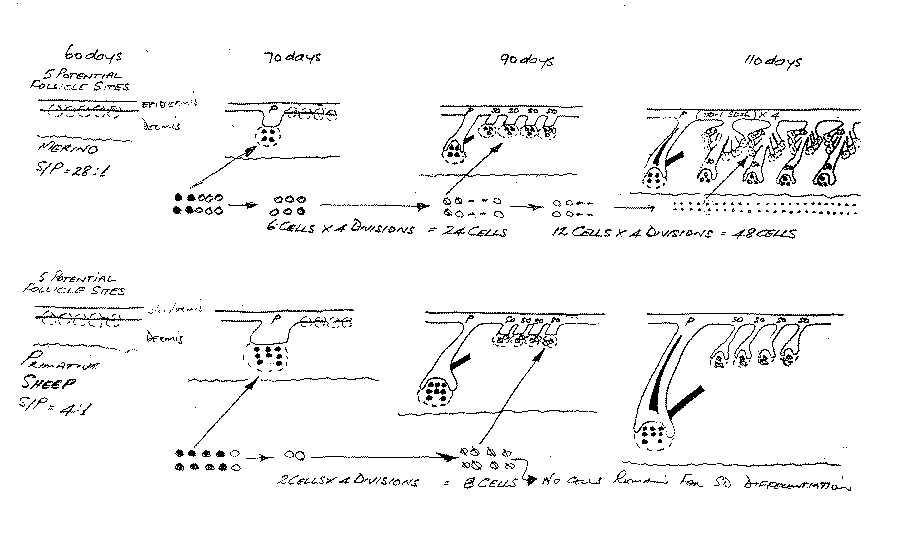
\includegraphics[width=1.9\textwidth,trim = 20 0 0 80]{images/fig16.png}
  \caption{  A quantitative illustration of predictions which can be made with
      the Moore hypothesis regarding the role of primary follicle size
      in determining comparative development of Merino and primitive
      foetal skin over the period 60-110 days of gestation.  Note that
      this presentation is diagrammatic - relative sizes and shapes of
      follicles are not able to accurately represent reality, and cell
      numbers and division rates should not be taken to be absolute.
      For a complete explanation see text.}
  \label{fig:16}
\end{figure}
\end{landscape}

%\end{document}


    Take an arbitrary area of skin containing 5 potential initiation sites
and 10 pre-papilla cells, in both Merino and primitive, at some time prior to
70 days.  Let the cell division rate (of pre-papilla cells) be 4 divisions per
20 days in both Merino and primitive.  At 70 days let the Merino develop one
primary follicle, using 4 pre-papilla cells and one site;  let the primitive
also develop one primary follicle, but using 8 pre-papilla cells and one site. 
Let this difference (4 versus 8 cells) be the only pre-determined difference
between the two development processes.
    In the Merino development continues as follows:  the 6 remaining pre-
papilla cells divide to form 24 cells over the period 70-90 days.  At 90 days,
4 SO follicles form, using 3 pre-papilla cells each and the 4 remaining sites,
leaving 12 cells undifferentiated.  The twelve remaining cells divide again
over 90-110 days, making 48 cells.  At 110 days, 24 SD follicles form using
2 pre-papilla cells each, and exhausting the supply pre-papilla cells, thus
halting follicle formation.  Because all sites were used at 70 days the SD
follicles form as branches from existing sites, mainly the S0 sites, thus
forming branching or compound follicles.  There are 28 (SD + S0) follicles
altogether, giving an adult S/P ratio of 28:1, typical of a Merino-like skin.
    In the primitive sheep development proceeds as follows.  The 2 remaining
pre-papilla cells divide to form 8 cells over the period 70-90 days.  At 90
days 4 SO follicles form, using 2 pre-papilla cells each, and the 4 remaining
sites.  There are no pre-papilla cells remaining, so development ceases, no
SD follicles being formed.  There are 4 (SD + S0) follicles altogether, giving
an adult S/P ratio of 4:1, typical of a primitive skin with coarse hair and
fine down.
    There are obviously shades of grey between the extremes illustrated. 
In reality all secondary follicles are not of equal size, or equal number of
symmetrically arranged branches, as shown in Figure 16.  It would detract from
comprehension to show such variation.
    We postulate that, during evolution of the Merino, a resource (the
population of pre-papilla cells) has been redirected by selective forces from
forming large primary follicles to forming many compound secondary follicles. 
The key observation is that the initial event (formation of the  primary
follicle) in this developmental process influences its later course.  We
therefore conclude that adult Dp is an observation representing the earliest
event of the follicle development process which we can measure, and suggest
it is likely to be the basic cause of the quantum difference between the
Merino and other breeds in fleece quality characteristics.  This is a
modification of the view of Dr Carter, who suggested that S/P ratio was the
basis of the difference between Merino and other breeds 
(Carter and Clarke~\cite{cart:57a}~\cite{cart:57b}). 
Our view is that differences in S/P are a consequence of earlier
differences in Dp.  It would be quite likely that the original Merino occurred
as a mutant gene with a major effect on primary follicle and fibre size, and
that its effect was subsequently masked by selection of modifying genes, so
that its segregation is not now obvious in crosses.  Genes of similar effect
occur in other species (Fraser~\cite{fras:53};  Searle and Jude~\cite{sear:56}) and are commonly
known as {\em rex} mutants.  If the Merino is a {\em rex} mutant sheep
it should be
possible to make its segregation visible in crosses by selecting Merinos in
a way which would suppress the action of modifying genes.  A new CSIRO
experiment (no. 73) may allow us to test this prediction.
    Conversely, if the  {\em rex} hypothesis is accepted, one would not expect
pure Merino populations to exhibit segregation at the {\em rex} locus, so
segregation could not be used to explain occurrence of primitive individuals
in purebreds.  Purebreds may have other modifying genes segregating, but these
would be more than one and small in effect.

\clearpage
\subsection{Evidence from Historical Accounts of Incidence od Primitive 
Individuals in Spanish Merino Flocks}
    There is some evidence that the original Merino flocks in Spain had an
incidence of primitive hairy individuals.  An anonymous author, discussing
Merino lambs introduced into England from Spain (A Practical Treatise on the
Merino and Anglo-Merino Breeds of Sheep, London, 1809;  cited by 
Ryder~\cite{ryde:86} ), states that:
\begin{quotation}
    'There is occasionally a peculiarity in the wool of the lamb when
    first dropped, differing from any breed in this country (if
    indeed it may be termed wool), many of them being entirely
    covered with hair, which I do not find mentioned by any author
    except Dr Parry (Communication to Board of Agriculture, vol. 5,
    p. 346) who observed that the wool of Merino lambs, in general,
    is evidently coarser and harder than that of the sheep.  It
    seems, however, that the different flocks vary in this respect. 
    The lambs of the Infantado and Paular races are covered with a
    coarse sort of hair, which afterwards changes into very fine
    wool.  The same appearance is sometimes to be found among lambs
    of the Negrete breed in England.'
\end{quotation}
    The above account does not mention hairy adult fleeces, but the
association of adult Dp with birthcoat is very strong in our data (Table~\ref{tb:8}),
so there is a high probability Spanish Merinos were also hairy as adults.
    There is also one piece of direct evidence.  There is a flock of Merinos
at La Bergerie Nationale, Rambouillet, France, that descend from Spanish
Merinos imported by the French Government in 1786.  Their history is described
by Carter~\cite{cart:79} and Ryder~\cite{ryde:86}. 
They would appear to be a large
representative sample of 18th century Spanish Merinos, maintained without
introductions.  In 1964 Dr Carter sampled 6 rams and 18 ewes from this flock. 
These data are still preserved at CSIRO, and are summarised in Table~\ref{tb:9}.

%\documentclass{article}
%\usepackage{lscape}
%\begin{document}

\begin{landscape}
\begin{table} 
\centering
\caption{Variation in Diameter of Primary and Secondary Fibres and in Percentage
	 of Follicles Exhibiting Shedding, in Sheep from the Merino Flock at
	 la Bergerie Nationale, Rambouillet, France}
%	 (sampled br Dr H. B. Carter~\cite{cart:68} in 1964).}
\label{tb:9} 
\vspace{0.1in}

\begin{tabular}{l|rrr|rrr|rr}  \hline
  Sex & \multicolumn{3}{c|}{Mean} &  \multicolumn{3}{c|}{Percent with Dp/Ds} & \% Shed &  Number \\ \cline{2-7}
      & Dp & Ds & Dp/Ds &   $>1.2$ &  $>1.5$ & $>1.8$ & Follicles & Sampled \\ \hline


Rams  & $19.4\pm1.02$ & $19.3\pm0.41$ & $1.00\pm0.32$  & 0.0  & 0.0 &  0.0 & $2.6\pm1.97$  &  6    \\
                                                                                 
Ewes  & $21.5\pm0.41$ & $19.1\pm0.29$ & $1.13\pm0.03$  & 38.9 &  0.0 &  0.0 & $0.6\pm0.37$ &  16    \\ \hline


\end{tabular}
\end{table}
\end{landscape}

%\end{document}


There
was one ram with 12.4% of shed follicles, and one ewe with Dp/Ds ratio of 1.44
(Dp = 25.1, Ds = 17.6).  These results are remarkably similar to the Early
Fine Merino in Table~\ref{tb:2}, and to the modern fine and medium non-Peppin Merinos
in Tables~\ref{tb:2}~and~\ref{tb:3}.  While one should always be cautious with such comparisons
of flocks in different environments, it suggests that Merino populations from
the present Australian strains to the original Spanish, have an ability to
generate individuals which resemble their primitive two coated ancestors.
    It is improbable that the flock at Rambouillet were subjected to
introductions of Cape or Bengal sheep but there may have been introductions
of the local European Breeds.  If it is possible for the Rambouillet flock to
exhibit primitive characteristics without such introductions, it is not
necessary to postulate such introductions into the finer Australian strains
of Merino, in order to explain a similar level of primitive characteristics.
    Hence, we suggest, most of the primitive characteristics which we
observe in today's Australian Fine Merino, came from the Spanish Merino and
its ancestors.  The Cape and Bengal sheep which came to Australia with first
settlement (Turner~\cite{turn:80}; Turner~\cite{turn:85};
Garran and White~\cite{garr:85};  Massy~\cite{mass:90},
 and/or introduction of British longwools (Cox~\cite{cox:36}; 
 Massy~\cite{mass:90}),
may have contributed additional primitive characteristics to the Medium,
Medium Peppin and Strong Merino strains.
    From the point of view of the hypothesis put forward in this paper, ie
that current Australian Merinos are descended from primitive two-coated sheep,
it does not matter whether there is one line of descent through pure breeding
or several lines of descent through various introductions.  All of the
documented historical introductions were also descended from primitive two-
coated sheep.

\clearpage
\subsection{Direct Evidence of Increased Incidence of Primitive 
Characteristics in a Feral Merino Population}
  The feral sheep of Arapawa Island, New Zealand, are considered to be
descendents of "the commercial Merinos of the 19th century", there being no
record of the introduction of any other breed to the region (Orwin and
Whitaker~\cite{orwi:84}).
Records of their presence on the island date back to the
1850's.  Their blood types are not inconsistant with a Merino origin.
    Orwin and Whitaker~\cite{orwi:84} report measurements of wool and skin from
Arapawa Island feral sheep.  Compared with modern Merinos they produce wool
high in grease content, bulk, and fibre crimp, but of similar diameter (mean
23.1�, median 21.6�).  In these characteristics they resemble Merinos more
than other commercial breeds.  However their fibre diameter distributions are
markedly skewed (range 9-109�m) and they have a low S/P ratio (6.0) a low
follicle density (26.9 per mm2) and have a tendency to shed their fleece.  In
these characteristics they resemble primitive breeds.
    Orwin and Whitaker~\cite{orwi:84} 
    present comparative data on four other feral
flocks, but in these cases strong evidence of Merino origin is lacking.  They
also refer to other feral Merino populations in Hawaii, the Solomon Islands,
but comparative data are not available.
    There is ample evidence that geographically isolated feral populations
evolve in the direction favoured by natural selection.  What the above
evidence establishes, in addition, is that in the case of Merino sheep
populations, natural selection for coat type regresses the population toward
the two-coated condition exhibited by primitive ancestors of the Merino.
    What remains to be established is whether, or at what rate, the same
phenomenon occurs in domestic Merino populations.



\clearpage
\section{Conclusion}
    The economic significance of primitive characteristics is difficult to
establish.  Whiteley~\cite{whit:87} 
rates fibre diameter variability, as a parameter
affecting product value, to be important only when certain limits are
exceeded.  He does not, however, define the critical limits, and he considers
only the effect on processing wastage.  Recent work at CSIRO, Division of
Textile Industry (Mayfield~\cite{mayf:87}; Garnsworthy~\cite{garn:88} 
shows that prickle in
fabrics is the result of an excess of coarse fibres, a small percentage of
fibres exceeding 30 microns in a fabric of mean diameter 21 microns being
sufficient to cause discomfort in a fabric worn against the skin.  Product
quality is therefore predicted from fibre diameter distribution.  Handle of
raw wool and of wool in various stages of processing is also predicted.  In
addition to these textile implications there is an effect on staple structure,
fleece rot resistance, and blowfly strike (Watts~\cite{watt:81}) which in turn
indirectly affect processing and product quality.  There is a need to define
these relationships with greater precision, and to make an assessment of the
economic importance of primary fibre diameter, relative to that of other
fleece characteristics.  An extension of the work of 
Whitely and Jackson~\cite{whit:81}
and Rogan~\cite{roga:88} is indicated.
    There is also a need to understand how primary and secondary fibre
diameter distributions relate to other assessments of quality which are
traditionally made on the live sheep.  We have preliminary evidence (Lax,
unpublished) to suggest that sheep classers can accurately assess occurrence
of coarse fibres in the fleece from a combination of handle and visual fleece
characteristics.  This suggests that practical and economically feasible
methods of selecting against hairiness already exist in the industry, and in
many cases we believe that such methods are being applied with sufficient
diligence and persistance.  The worst hairiness problems were observed in
selection experiments (which are selected entirely on objective measurement),
in control flocks (in which there is no selection at all), and in certain
studs which have dispensed with the traditional safequards which are built
into visual classing.  The positive result is that there are some studs that
have successfully combined objective measurement with traditional culling for
faults such as hairiness.  These flocks are relatively free of excessively
hairy individuals.  It is to these breeders that we should look for assistance
in integrating the new {\em sharp} tools offered by objective measurement with the
traditional {\em cautious} approach of visual assessment.  For reasons of
confidentiality we are obliged not to identify the studs which were involved
in assembling the above observations.  We conclude that some selection against
hairiness is essential in any Merino breeding program.
    None of the above interpretations explain why sheep with primitive hairy
fleeces continue to occur in Australian Merino flocks.  We only know that it
is necessary to exert a certain amount of selective force in order to prevent
their occurrence reaching unacceptable levels.  Exactly how much selection is
required against hairiness has yet to be determined.  The answer is unlikely
to be the same for all strains.  One leading breeder has advised
confidentially that he expends about 30\% of his available selection intensity
in culling against hairiness.  When so much culling is required, it is a major
problem diverting selection effort away from important production traits.  The
only way to eliminate such a problem is to understand the biological basis of
undesirable genetic correlations.  We have taken one small step towards that
understanding, in the case of correlations between hairiness and production
traits, firstly by demonstrating that a problem exists (though its extent has
yet to be quantified) and secondly by exploring evolutionary and developmental
explanations.  The outstanding question which remains unanswered is why Dp
should be positively correlated with reproductive fitness.  Its association
with lamb survival, via birthcoat, is well documented 
(Alexander~\cite{alex:62};  Obst~\cite{obst:70}),
but the only reported association of coat type with adult performance
is in the rock squirrel (Walsberg~\cite{wals:88})
where solar heat gain was found to
be minimized by a particular ratio of inner to outer coat depths, the outer
coat being entirely coarse primary fibres.  It may not be entirely
unreasonable to suggest that coat type in sheep has an effect on
thermoregulation;  fur and warm blooded metabolism evolved together and may
well be genetically linked even if there is no direct physical effect.  The
link between thermoregulation and reproductive performance is well documented. 
Heat stress affects semen quality, embryonic loss, foetal growth and lamb
survival (Brown and Hutchinson~\cite{brow:73}).
There are also documented effects of
heat and cold stress on adult wool production and quality (Wodzicka, 1960; 
Slee and Ryder~\cite{slee:67};  Downes~\cite{down:69}).
Of particular interest is an effect of
heat stress of the pregnant ewe on secondary follicle maturation of the lamb
(Cartwright~\cite{cart:76}).
The field was reviewed by Bottomley~\cite{bott:79}.  We suggest
that genetic association between coat type and thermoregulation in sheep
merits further investigation.  The adaptive significance of coat type could
be an important consideration in the formation of sheep breeding objectives
for various parts of the Australian continent.
    It should not be assumed that all of the observations reported here are
either new or original.  Our interpretation of the observations may vary from
that of previous workers, but the fact of occurrence of individuals of
primitive coat type in Merino flocks is widely known throughout the industry,
as the following citation from Country Life of 18 October 1932 clearly
demonstrates.
\begin{quotation}
    'A freak Merino ram has come into the possession of the
    Department of Agriculture - a freak because of its extraordinary
    wool growth, which is said to have a coating similar to the
    original wild sheep.  This freak ram - now at Trangie Experiment
    Farm - is a rising 4 tooth.  Mr E A Elliot, Government Sheep and
    Wool Expert, told the writer that it will be used for breeding
    purposes, in order to see whether it will reproduce its kind. 
    The ram was bred in a high class stud flock and because of this
    fact will be joined with selected Merino ewes.  In addition to
    having a coating of short wool and hair, the ram is very leggy
    and has practically no fold development.  The ram, too, has a
    thick jaw, and is very active ...'
\end{quotation}
    This account was quoted by Cox~\cite{cox:36} 
    who also presents a photograph of
the ram clearly showing the short fleece with protruding hair.  The context
of Cox's citation show that he considers this {/em freak} an example of
reappearance of a primitive breed characteristic.  There seems to be no record
of further research into this animal or its progeny.  It is somewhat
surprising that a phenomenon widely publicized could be ignored in breeding
research for four decades.
    The only definite result of this study is a confirmation that sheep with
primitive skin and fleece characteristics do exist in the current Australian
Merino population, and have probably always been present in the Merino breed. 
We interpret this observation as consistent with Ryder's theory of evolution
of the Merino directly from primitive two-coated domestic sheep.  This
interpretation led us to the hypothesis that Merino flocks tend to regress
toward wild or primitive sheep, at least in so far as their coat type is
concerned.  The conditions under which this tendency is actualized would
appear to be fairly common. 


\clearpage
\begin{thebibliography}{99}

\bibitem{alex:62}
Alexander, G. (1962).  Temperature regulation in the newborn lamb. IV. The
    effect of wind and evaporation of water from the coat on metabolic rate
    and body temperature.  Aust. J. Agric. Res. 13, 82-89.
\bibitem{barl:74}
Barlow, R. (1974).  Selection for clean fleece weight in Merino sheep.  II
    Correlated responses to selection.  Aust. J. Agric. Res. 25: 973-94.
\bibitem{bott:79}
Bottomley, G.A. (1979).  "Weather and wool growth".  In:  Physiological and
    Environmental Limitations to Wool Growth .  Ed. J.L. Black and
    P.J. Reis.  Proceedings of a National Workshop, Leura, NSW, Australia,
    April 1978.  
\bibitem{brow:73}
Brown, G.D. and Hutchinson, J.C.D. (1973).  Climate and animal Production. 
    In:  The Pastoral Industries of Australia.  Ed. G. Alexander and
    O.B. Williams.  Sydney University Press, Sydney.
\bibitem{brow:68}
Brown, G.D. and Turner, H.N. (1968).  Response to selection in Australian
    Merino sheep.  II. Estimates of phenotypic and genetic parameters for
    some production traits in Merino ewes and an analysis of the possible
    effects of selection on them.  Aust. J. Agric. Res. 19: 303-22.
\bibitem{cart:55}
Carter, H.B. (1955).  The hair follicle group in sheep.  Anim. Breed. Abstr.
    23, 102.
\bibitem{cart:65}
Carter, H.B. (1965).  Variation in the hair follicle population of mammalian
    skin.  In:  Biology of the Skin and Hair Growth.  Ed. A.G. Lyne and
    B.F. Short.  Angus and Robertson, Sydney, 1965.
\bibitem{cart:68}
Carter, H.B. (1968).  Comparative Fleece Analysis Data for Domestic Sheep. 
    The Principal Fleece Staple Values of some Recognized Breeds.
    Agricultural Research Council.
\bibitem{cart:79}
Carter, H.B. (ed.) (1979).  The Sheep and Wool Correspondence of Sir Joseph
    Banks 1781-1820.  Library Council of NSW and B.M. (Nat. Hist.).
\bibitem{cart:57a}
Carter, H.B. and Clarke, W.H. (1957a).  The hair follicle group and skin
    follicle population of Australian Merino sheep.  Aust. J. Agric. Res.
    8, 91-108.
\bibitem{cart:57b}
Carter, H.B. and Clarke, W.H. (1957b).  The hair follicle group and follicle
    population of some non-Merino breeds of sheep.  Aust. J. Agric. Res. 8,
    109-19.
\bibitem{cart:76}
Cartwright, G.A. and Thwaites, C.J. (1976).  J. Agric. Sci. 86, 581.
\bibitem{cox:36}
Cox, E.W. (1936).  The Evolution of the Australian Merino.  Angus and
    Robertson Limited, Sydney
\bibitem{coy:79}
Coy, J. (1979).  In: Composite Transcript of Sheep Breeding Workshops. 
    Ed. N.M Elliot.  Department of Agriculture, Bairnsdale, Victoria, 
    30 April - 4 May, 1979.
\bibitem{down:69}
Downes, A.M. and Hutchinson, J.C.D. (1969).   Effect of low skin surface
    temperature on wool growth.  J. Agric. Sci. Camb. 72, 155-58.
\bibitem{fras:53}
Fraser, A.S. (1953).  A note on the growth of the Rex and Angora coats.     
    J. Genetics 51, 237-42.
\bibitem{fras:60}
Fraser, A.S. and Short, B.F. (1960).  The Biology of the Fleece.  CSIRO
    Animal Research Labs.  Technical Paper No. 3.
\bibitem{gall:70}
Gallagher, J.R. (1970).  An evaluation of Merino wool quality.  II. An
    estimate of the incidence of coarse fibres in Australian Merino wool. 
    J. Agric. Sci. Camb. 74, 99-102.
\bibitem{gall:70a}
Gallagher, J.R. and Yeates, N.T.M. (1970).  An evaluation of Merino wool
    quality.  I. The incidence of coarse fibres in two Australian Merino
    flocks.  J. Agric. Sci. Camb. 74, 91-98.
\bibitem{garn:88}
Garnsworthy, R.K., Gully, R.L., Kandiah, R.P., Kenins, P., Mayfield, R.J. and
    Westerman, R.A. (1988).  Understanding the Causes of Prickle and Itch
    from the Skin Contact of Fabrics.  CSIRO, Division of Wool Technology,
    Report No. G64.  Belmont, Victoria.
\bibitem{garr:85}
Garran, J.C. and White, L. (1985).  "Merinos, myths and Macarthurs".  Aust.
    National Uni. Press. Pergamon Press, Sydney.
\bibitem{hard:56}
Hardy, M.H. and Lyne, A.G. (1956).  The pre-natal development of wool
    follicles in Merino sheep.  Aust. J. Biol. Sci. 9, 423-41.
\bibitem{hoga:79}
Hogan, J.P., Elliot, N.M. and Hughes, A.D. (1979).  "Maximum wool growth
    rates expected from Australian Merino".  In:  Physiological and
    Environmental Limitations to Wool Growth.  Ed. J.L. Black and P.J.
    Reis.  Proceedings of a National Workshop, Leura, NSW, Australia, April
    1978.
\bibitem{ibra:82}
Ibrahim, L. and Wright, E.A. (1982).  As quantitative study of hair growth
    using mouse and rat vibrissal follicles.  J. Embrol. Exp. Morphol. 72,
    209-224.
\bibitem{jack:90}
Jackson, N. and Maddocks, I.G.  Automatic evaluation of follicle number and
    fibre diameter in transverse sections of sheep skin.  Zeiss
    Information.  Submitted 1990.
\bibitem{lyne:57}
Lyne, A.G. (1957).  Bundles of primary wool follicles in sheep.  Nature 179,
    825-826.
\bibitem{madd:88}
Maddocks, I.G. and Jackson, N. (1988).  Structural studies of sheep, cattle
    and goat skin.  CSIRO, Division of Animal Production, Sydney.
\bibitem{mars:55}
Marston,   (1955)

\bibitem{maso:67}
Mason, I.L. (1967).  "Sheep Breeds of the Mediterranean".  Commonwealth
    Agricultural Bureau, Edinburgh.
\bibitem{mass:90}
Massy, C. (1990).  "The Australian Merino". Viking-O'Neil.
\bibitem{mayf:87}
Mayfield, R. (1987).  Clothing Physiology - Preventing Prickle.  Textile
    Horizons, pp. 35-6, November 1987.
\bibitem{moor:84}
Moore, G.P.M. (1984).  "Growth and Development of Follicle Populations and
    Critical Stages of Growth".  In:  Wool Production in Western Australia. 
    Eds S.K. Baker, D.G. Masters and I.H. Williams.  Proceedings,
    pp. 69-76.
\bibitem{moor:84a}
Moore, G.P.M. and Jackson, N. (1984).  An hypothesis implicating a founder
    cell population in the regulation of wool follicle formation and
    distribution in sheep skin.  J. Embryol. Exp. Morph. 82 (Suppl.), 259.
\bibitem{moor:89}
Moore, G.P.M., Jackson, N. and Lax, J. (1989).  Evidence of a unique
    developmental mechanism specifying follicle density and fibre size in
    sheep selected for single skin and fleece characters.  Genetical
    Research.  53, 57-62.
\bibitem{morl:55}
Morley, F.H.W. (1955).  Selection for economic characters in Australian
    Merino sheep.  V. Further estimates of phenotypic and genetic
    parameters.  Aust. J. Agric. Res. 6, 77-90.
\bibitem{nay:73}
Nay, T. (1973).  Wool Follicles - A Manual for Breeders.  Aust. Wool Corp.,
    Melbourne.
\bibitem{obst:70}
Obst, J.M. and Evans, J.V. (1970).  Genotype-environment interactions in lamb
    mortality with particular reference to birthcoat and haemoglobin type. 
    Proc. Aust. Soc. Anim. Prod. 8, 149-58.
\bibitem{orwi:84}
Orwin, D.F.G. and Whitaker, A.H. (1984).  Feral sheep (Ovies aries L.) of
    Arapawa Island, Marlborough Sounds, and a comparison of their wool
    characteristics with those of four other feral flocks in New Zealand. 
    New Zealand J. Zoology 11: 201-224.
\bibitem{rawl:65}
Rawles, M.E. (1965).  Tissue interactions in the morphogenesis of the
    feather.  In:  Biology of the Skin and Hair Growth.  Ed.  A.G. Lyne and
    B.F. Short.  Angus and Robertson, Sydney 1965.
\bibitem{rend:78}
Rendel, J.M. and Nay, T. (1978).  Selection for high and low ratio and high
    and low primary density in Merino sheep.  Aust. J. Agric. Res. 29,
    1077-1086.
\bibitem{roga:88}
Rogan, I.M. (1988).  Genetic variation and covariation in wool
    characteristics related to processing performance and their economic
    significance.  Third World Congress on Sheep and Beef Cattle Breeding,
    Paris, June 1988.
\bibitem{ruda:55}
Rudall, K.M. (1955).  The size and shape of the papilla in wool follicles. 
    Proc. Int. Wool Textile Res. Conf. Aust., 1955, vol. F, pp. 9-25.
\bibitem{ryde:58}
Ryder, M.L. (1958).  Follicle arrangement in skin from wild sheep, primitive
    domestic sheep and in parchment.  Nature 182, 781-83.
\bibitem{ryde:64}
Ryder, M.L. (1964).  Fleece evolution in domestic sheep.  Nature 204,       
    555-59.
\bibitem{ryde:66}
Ryder, M.L. (1966).  Coat structure in Soay sheep.  Nature 211, 1092-93.
\bibitem{ryde:86}
Ryder, M.L. (1986).  Sheep and Man.  Duckworth, London.
\bibitem{schi:58}
Schinckel, P.G. (1958).  The relationship of lamb birthcoat to adult fleece
    structure in a strain of Merino sheep.  Aust J. Agric. Res 9, 567-78.
\bibitem{sear:56}
Searle, A.G. and Jude, A.C. (1956).  The {\em Rex} type of coat in the domestic
    cat.  J. Genetics 54, 506-13.
\bibitem{shor:58}
Short, B.F., Fraser, A.S. and Carter, H.B. (1958).  Effect of level of
    feeding on the variability of fibre diameter in four breeds of sheep. 
    Aust. J. Agric. Res. 9, 229-36.
\bibitem{slee:67}
Slee, J. and Ryder, M.L. (1967).  The effect of cold exposure on wool growth
    in Scottish Blackface and Merino x Cheviot sheep.  J. Agric. Sci.
    (Camb.) 60, 449-53.
\bibitem{turn:80}
Turner, Helen Newton (1980).  "Origins of the CSIRO Booroola".  In: The
    Booroola Merino.  Ed. L.R. Piper, B.M. Bindon and R.D. Nethery. 
    Proceedings of Workshop, Armidale, NSW, 24-25 August, 1980.  
\bibitem{turn:85}
Turner, H.N. (1985).  "The Value of Sheep and Goat Imports to Australia". 
    Proceedings of AAABG 5th Conf., Sydney 26-28 August, 1985, pp. 3-8.
\bibitem{turn:70}
Turner, H.N., Brooker, M.G. and Dolling, C.H.S. (1970).  Response to
    selection in Australian Merino sheep. III.  Single character selection
    for high and low values of wool weight and its components.  Aust. J.
    Agric. Res. 21, 955-984.
\bibitem{wals:88}
Walsberg, G.E. (1988).  The significance of fur structure for solar heat gain
    in the rock squirrel, Spermophilus variegatus.  J. Exp. Biol. 138,    
    243-57.
\bibitem{wats:77}
Watson, N., Jackson, N. and Whiteley, K.J. (1977).  Inheritance of the
    resistance to compression property of Australian Merino wool and its
    genetic correlation with follicle curvature and various wool and body
    characters.  Aust. J. Agric. Res. 28, 1083-94.
\bibitem{watt:81}
Watts, J.E., Merritt, G.C., Lunney, H.W.M., Bennett, N.W. and Dennis, J.A.
    (1981).  Observations on fibre diameter variation in sheep in relation
    to fleece-rot and body strike susceptibility.  Aust. Vet. J. 57,      
    372-76.
\bibitem{whit:87}
Whiteley, K.J. (1987).  Wool processing.  Wool Tech. Sheep Breed. 36,       
    109-13.
\bibitem{whit:81}
Whiteley, K.J. and Jackson, N. (1981).  Breeding for apparel wool.  Proc.
    World Congress of Sheep and Beef Cattle Breeding, Palmerston North, New
    Zealand, October-November, 1980.
\bibitem{wodz:60}
Wodzicka, M. (1960).  Seasonal varitions in wool growth and heat tolerance of
    sheep.  I. Wool growth.  Aust. J. Agric. Res. 11, 75-84.

\end{thebibliography}

\end{document}
